

\section{Chapter 2: Labor Supply}

The aggregate labor supply 
is the sum of the individual labor supply decisions
of all prospective workers in the economy.
This chapter will be focused on 
fleshing out the framework that economists use 
to think about labor supply decisions.

%%%%%%%%%%%%%%%%%%%%%%%%%%%%%%%%%%%%%%%%%%%%%%%%%%%%%%%%%%%%%%%%%%%%%%%%%%%%%%%%%%%%%%%
%%%%%%%%%%%%%%%%%%%%%%%%%%%%%%%%%%%%%%%%%%%%%%%%%%%%%%%%%%%%%%%%%%%%%%%%%%%%%%%%%%%%%%%
\subsection{Terms}

\begin{itemize}
    \item $LF$: The size of the labor force
    \item $E$: The number of employed individuals
    \item $U$: The number of unemployed individuals
    \item $P$: The size of the population
    \item $C$: The consumption of goods
    \item $L$: The consumption of leisure
    \item $U=f(C, L)$: The utility function
    \item $MU_L$: The marginal utility of leisure
    \item $MU_C$: The marginal utility of consumption
    \item $V$: Nonlabor income
    \item $h$: Hours worked
    \item $w$: The wage rate
    \item $T$: Total time available in, say, a week
    \item $\sigma$: The labor supply elasticity
\end{itemize}

%%%%%%%%%%%%%%%%%%%%%%%%%%%%%%%%%%%%%%%%%%%%%%%%%%%%%%%%%%%%%%%%%%%%%%%%%%%%%%%%%%%%%%%
%%%%%%%%%%%%%%%%%%%%%%%%%%%%%%%%%%%%%%%%%%%%%%%%%%%%%%%%%%%%%%%%%%%%%%%%%%%%%%%%%%%%%%%

\subsection{Measuring the Labor Force}

The CPS classified individuals over the 
age of 16 into three categories:

\begin{enumerate}
    \item Employed: Somebody working 
        at least 1 hour of paid labor or 15 hours of unpaid labor
    \item Unemployed: Somebody temporarily laid off 
        from a job or actively looking for work
    \item Out of the labor force: Everyone else
\end{enumerate}

\begin{definition}[Labor Force] 
    The labor force (LF) is everyone who is employed (E) or unemployed (U).

    \begin{align}
        L F=E+U
    \end{align}

\end{definition}

\begin{definition}[Labor Force Participation Rate] 

    The Labor Force Participation Rate is the fraction of the population (P) that is in the labor force.

    \begin{align}
        \text { Labor force participation rate }=\frac{L F}{P}
    \end{align}

\end{definition}


\begin{definition}[Employment Rate] 
    
    The fraction of the population that is employed.

    \begin{align}
        \text { Employment rate }=\frac{E}{P}
    \end{align}

\end{definition}

\begin{definition}[Unemployment Rate] 

    The fraction of the population that is unemployed.

    \begin{align}
        \text { Unemployment rate }=\frac{U}{L F}
    \end{align}
    
\end{definition}

Notice that the number of unemployed people is 
calculated as a fraction of the labor force,
not as a fraction of the population. Thus, one 
way for the unemployment rate to go down is 
for people to stop looking for work entirely.

%%%%%%%%%%%%%%%%%%%%%%%%%%%%%%%%%%%%%%%%%%%%%%%%%%%%%%%%%%%%%%%%%%%%%%%%%%%%%%%%%%%%%%%
%%%%%%%%%%%%%%%%%%%%%%%%%%%%%%%%%%%%%%%%%%%%%%%%%%%%%%%%%%%%%%%%%%%%%%%%%%%%%%%%%%%%%%%
\subsection{Basic Facts about Labor Supply}

Below are just a few facts of key labor supply trends
over the last century.
\autoref{fig:ch2p2_men_women}
shows the labor force participation rate
for men and women over the last century.
\autoref{fig:ch2p2_weekly_hours}
shows the average weekly hours worked
for all workers over the last century.

\FloatBarrier

\begin{figure}[!htb]
    \centering
        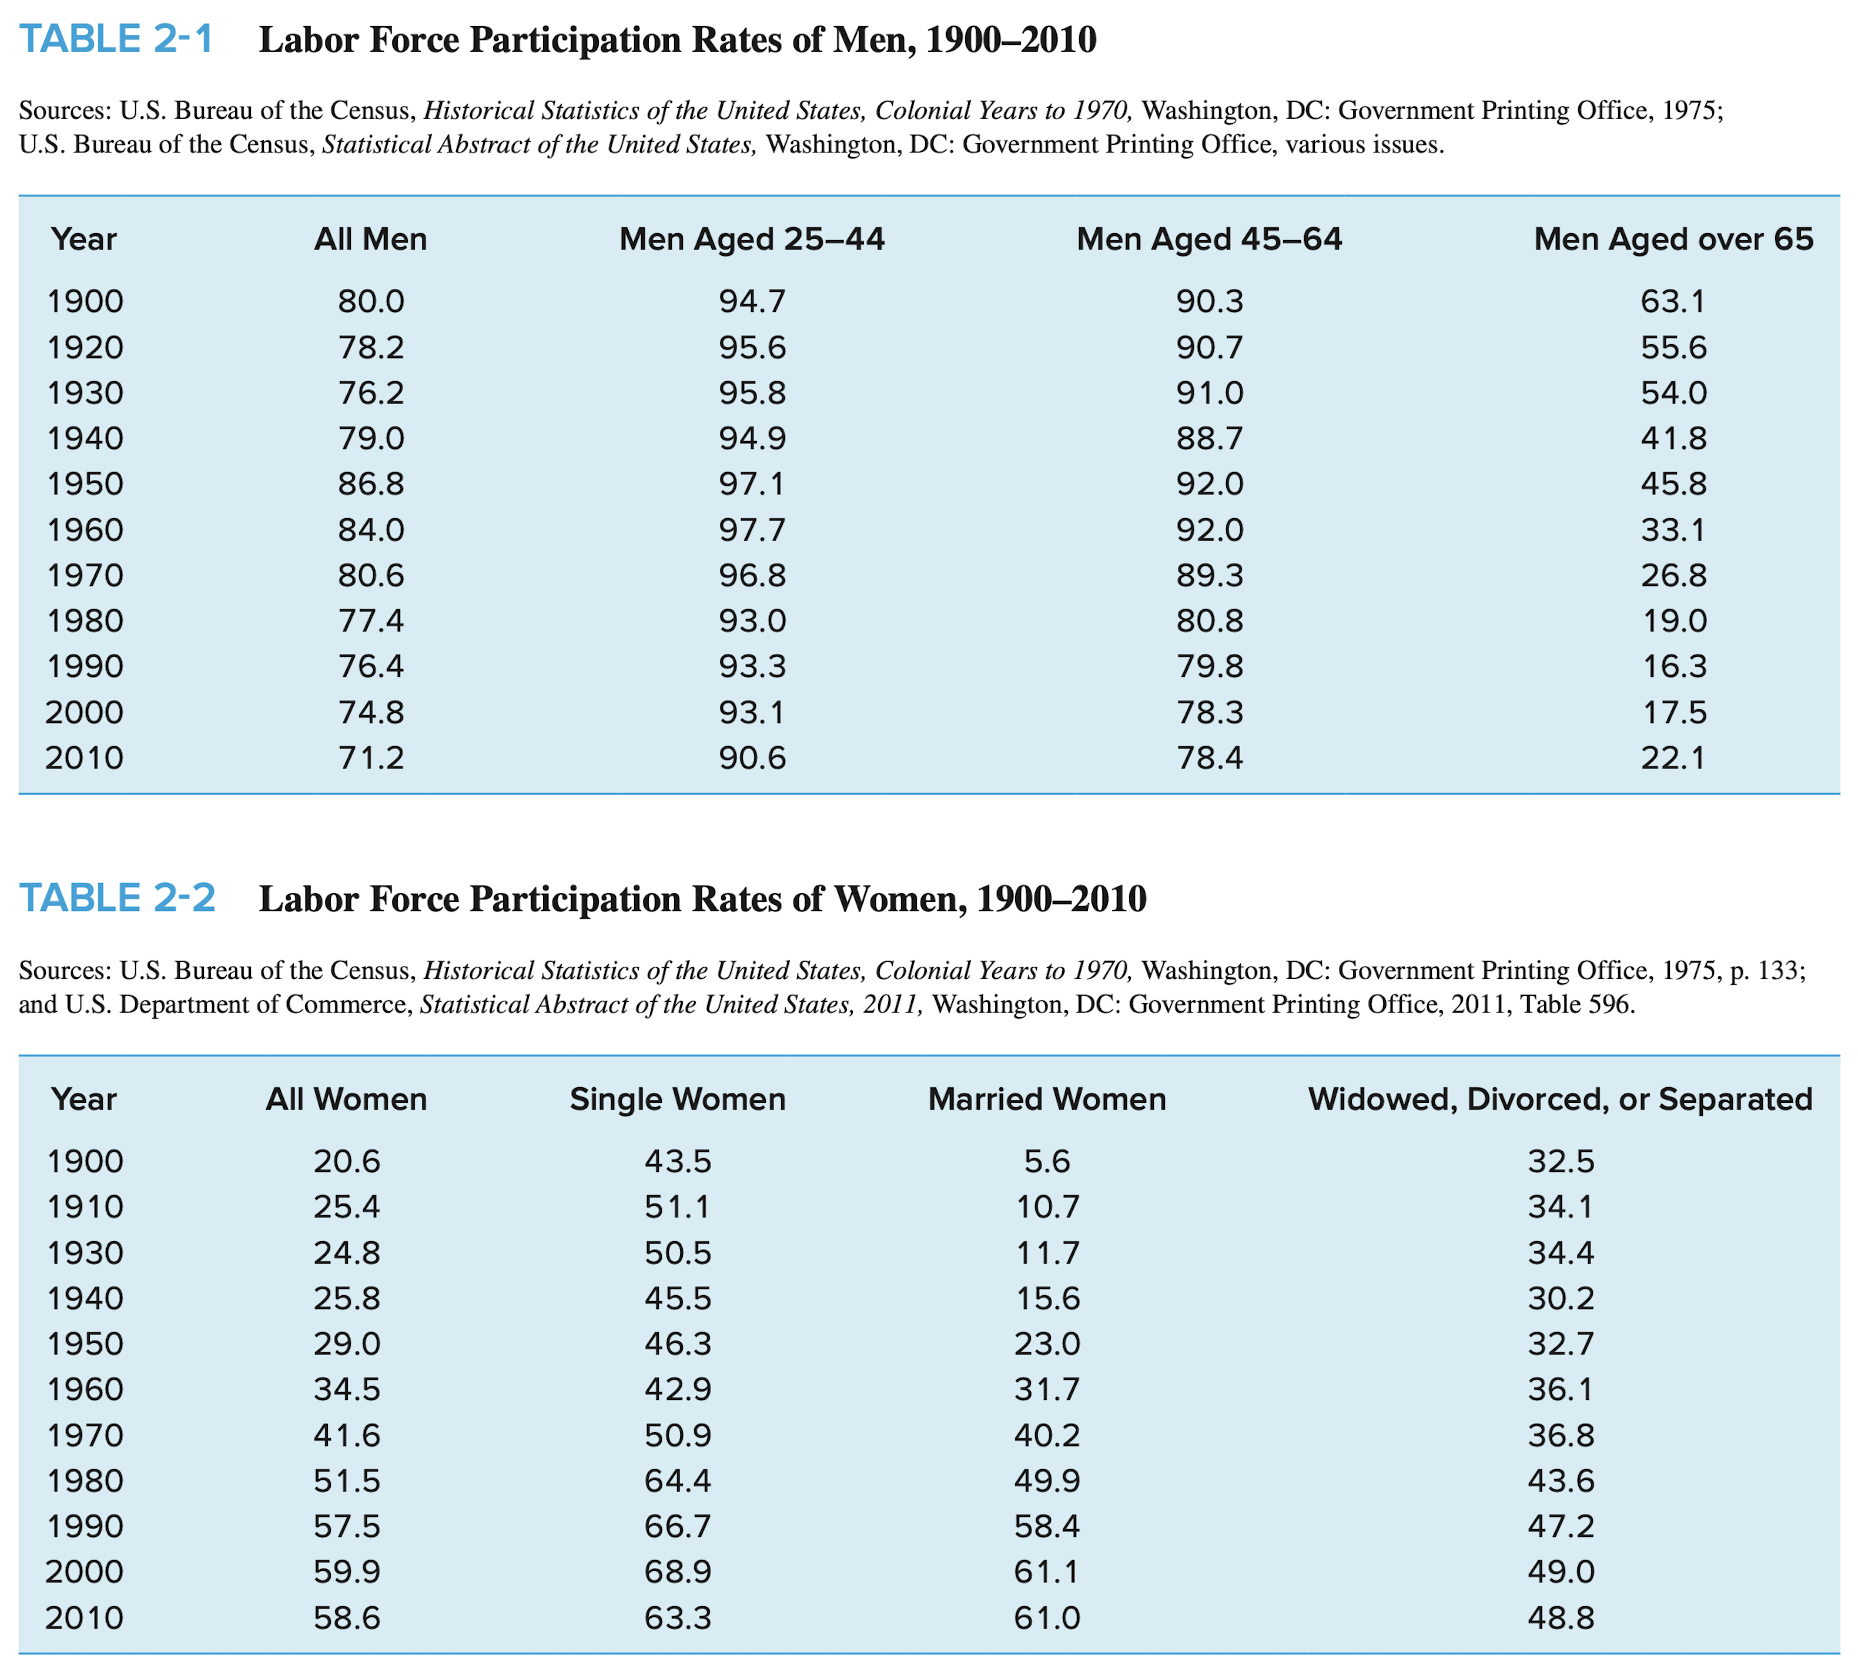
\includegraphics[width=0.95\textwidth]{../input/ch_2_tables_1_and_2.png}
    \caption{Labor Force Participation Rate for Men and Women}
    \label{fig:ch2p2_men_women}
\end{figure}

\begin{figure}[!htb]
    \centering
        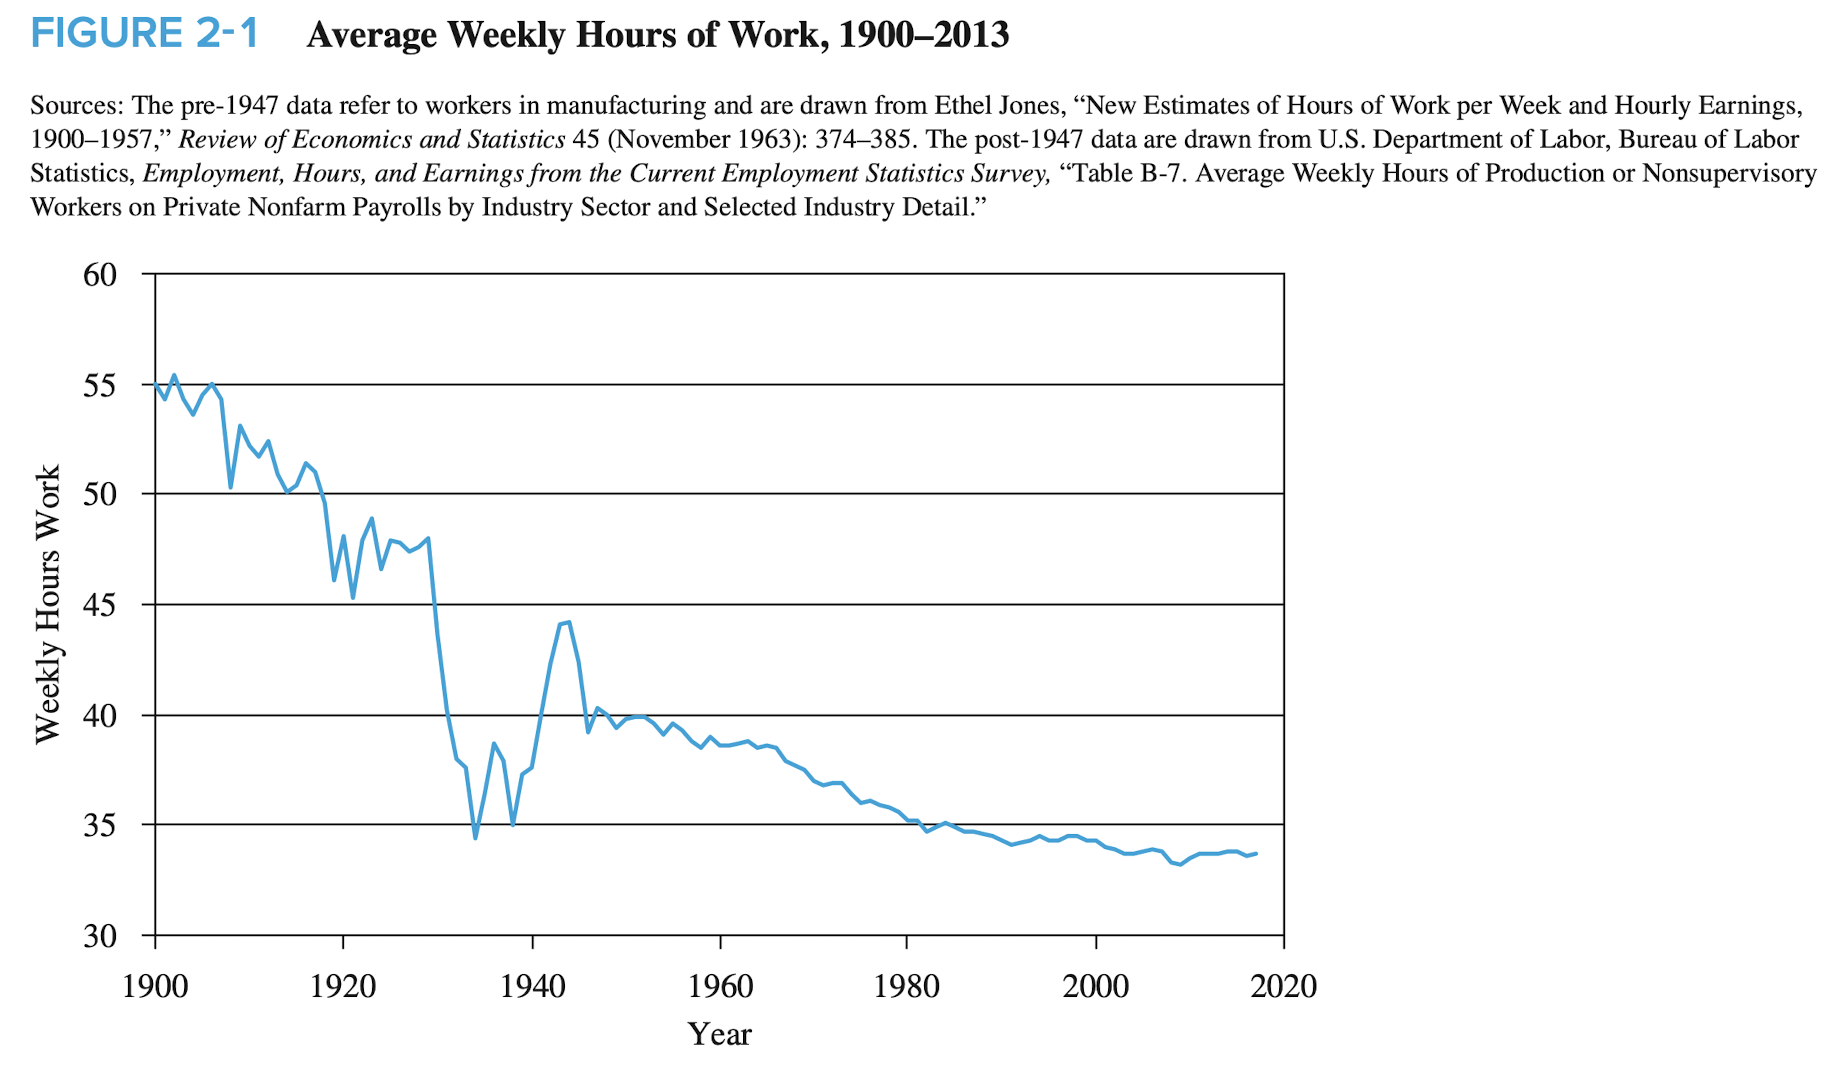
\includegraphics[width=0.95\textwidth]{../input/ch_2p2_weekly_hours.png}
    \caption{Average Weekly Hours Worked}
    \label{fig:ch2p2_weekly_hours}
\end{figure}

\FloatBarrier

%%%%%%%%%%%%%%%%%%%%%%%%%%%%%%%%%%%%%%%%%%%%%%%%%%%%%%%%%%%%%%%%%%%%%%%%%%%%%%%%%%%%%%%
%%%%%%%%%%%%%%%%%%%%%%%%%%%%%%%%%%%%%%%%%%%%%%%%%%%%%%%%%%%%%%%%%%%%%%%%%%%%%%%%%%%%%%%
\subsection{The Worker's Preferences}

The framework that economist's typically use
to think about labor supply behavior is the 
``neoclassical model of labor-leisure choice.''
This model is used to think about what's underpinning 
a worker's decision regarding whether and how much 
to work.

%%%%%%%%%%%%%%%%%%%%%%%%%%%%%%%%%%%%%%%%%%%%%%%%%%%%%%%%%%%%%%%%%%%%%%%%%%%%%%%%%%%%%%%

\subsubsection{Indifference Curves}

Under this model, we think of an agent as 
deriving utility from both
consumption ($C$) and leisure ($L$).
We express the utility function as
$U = f(C, L)$, where higher $U$ 
indicates higher utility and is 
preferred by the agent.

We use indifference curves to 
represent the combinations of $C$ and $L$
that yield the same level of utility.

See \autoref{fig:ch2p3_indifference_curve} 
for an example of indifference curves.

\FloatBarrier

\begin{figure}[!htb]
    \centering
        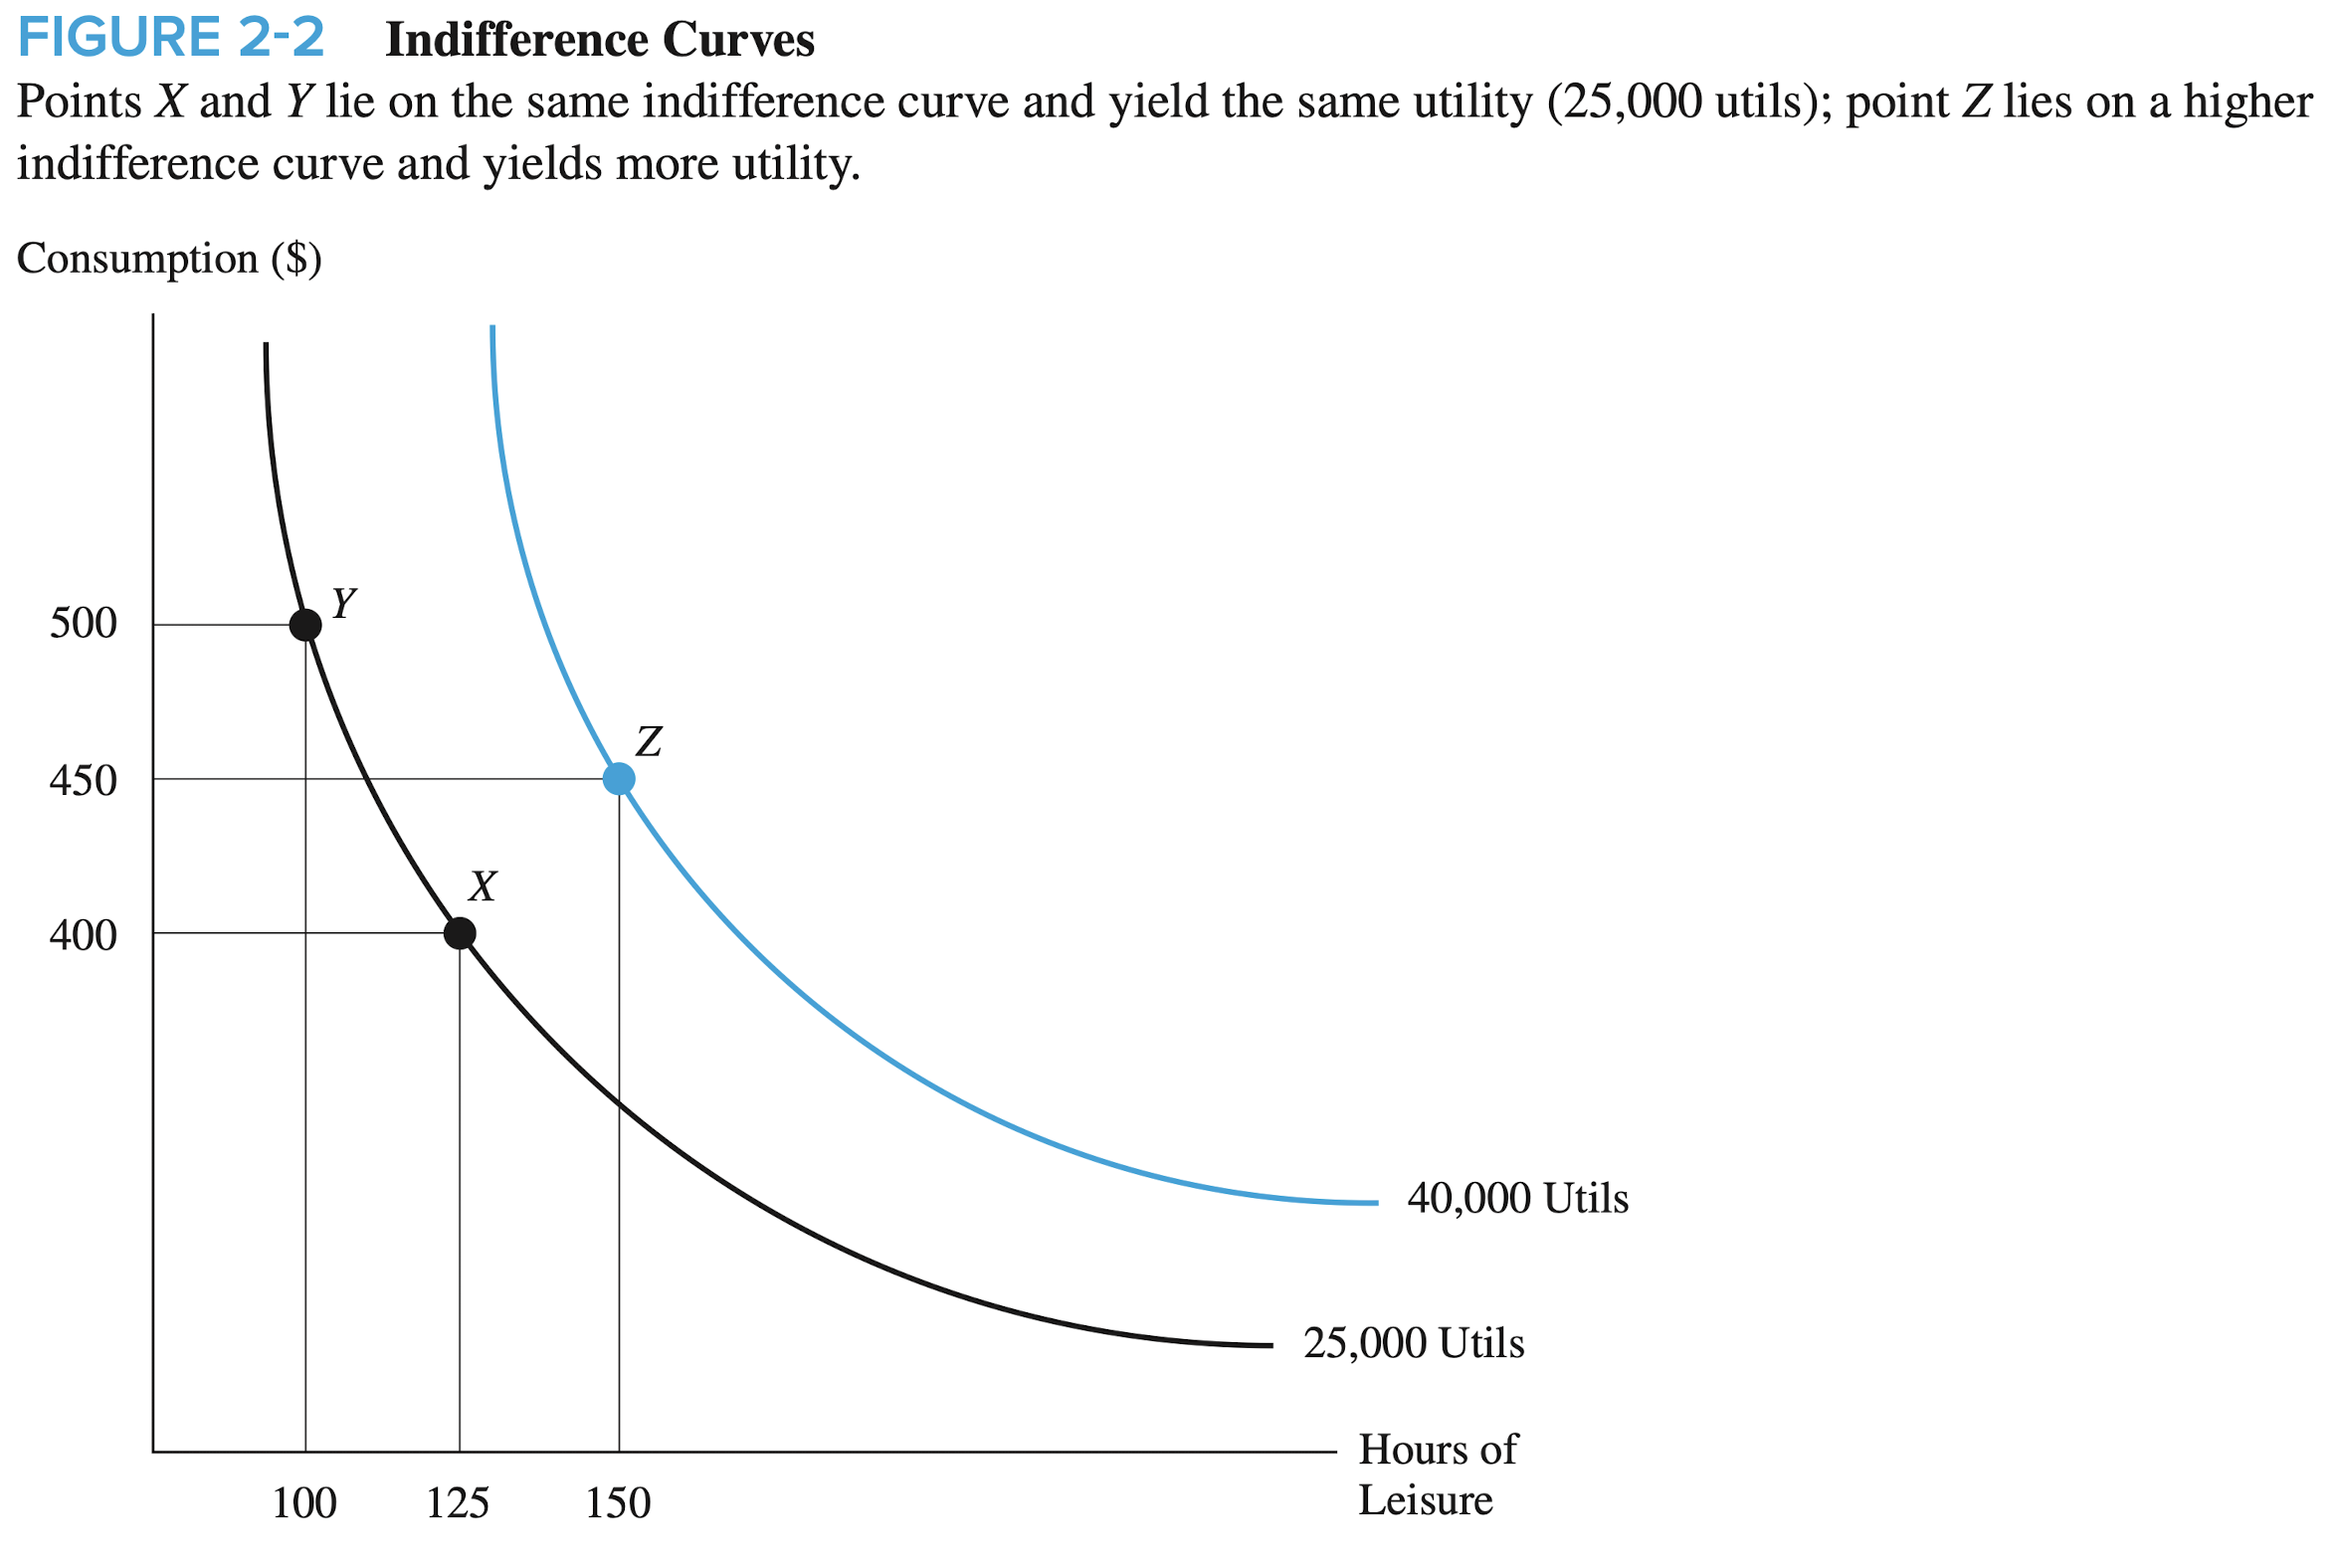
\includegraphics[width=0.9\textwidth]{../input/ch_2p3_indiff_curves.png}
    \caption{Indifference Curves}
    \label{fig:ch2p3_indifference_curve}
\end{figure}

\FloatBarrier

Indifference curves can be quite flexible 
in some aspects of their shape, but there
are four properties that we generally impose:

\begin{enumerate}
    \item Indifference curves are downward sloping: Otherwise, you 
        could get more of both $C$ and $L$ without getting any additional utility.
    \item Higher indifference curves indicate higher levels of utility
    \item Indifference curves don't intersect: Otherwise, one point 
        would yield two different levels of utility.
    \item Indifference curves are convex to the origin
\end{enumerate}

%%%%%%%%%%%%%%%%%%%%%%%%%%%%%%%%%%%%%%%%%%%%%%%%%%%%%%%%%%%%%%%%%%%%%%%%%%%%%%%%%%%%%%%
\subsubsection{The Slope of an Indifference Curve}

Marginal utility from an additional 
unit of consumption is denoted $MU_C$.
Similarly, the marginal utility from an additional 
unit of leisure is denoted $MU_L$.

The slope of an indifference curve is
given by

\begin{align}
    \frac{\Delta C}{\Delta L}=-\frac{M U_L}{M U_C}
\end{align}

This is logical, since the claim of indifference 
mandates that the utility change is equivalent
as you move along the curve, so it must be that

\begin{align}
    \left| \underbrace{\Delta C}_{\parbox[t]{2cm}{\raggedright \footnotesize \centering reduction in consumption}} \cdot \underbrace{M U_C}_{\parbox[t]{2cm}{\raggedright \footnotesize \centering marginal utility of consumption}} \right| = \left| \underbrace{\Delta L}_{\parbox[t]{2cm}{\raggedright \footnotesize \centering increase in leisure}} \cdot \underbrace{M U_L}_{\parbox[t]{2cm}{\raggedright \footnotesize \centering marginal utility of leisure}} \right|
\end{align}

That is, you're essentializing making the changes equivalent 
after scaling by their impact on utility.

\begin{definition}[Marginal Rate of Substitution (MRS) in Consumption] 
    
    The Marginal Rate of Substitution (MRS) in consumption
    is the absolute value of the slope of the 
    indifference curve.

    That is,

    \begin{align}
        M R S_{C L}=\frac{M U_L}{M U_C} = \left|\frac{\Delta C}{\Delta L}\right|
    \end{align}

\end{definition}

%%%%%%%%%%%%%%%%%%%%%%%%%%%%%%%%%%%%%%%%%%%%%%%%%%%%%%%%%%%%%%%%%%%%%%%%%%%%%%%%%%%%%%%
%%%%%%%%%%%%%%%%%%%%%%%%%%%%%%%%%%%%%%%%%%%%%%%%%%%%%%%%%%%%%%%%%%%%%%%%%%%%%%%%%%%%%%%
\subsection{The Budget Constraint}

Let

\begin{itemize}
    \item $V$: Nonlabor income
    \item $h$: Hours worked
    \item $w$: The wage rate
    \item $L$: Hours of leisure
    \item $T$: Total hours available in, say, a week
        \begin{align}
            T = L + h
        \end{align}
\end{itemize}

An individual's budget constraint can then be written in 
various ways:

\begin{align}
    C=&w h+V \\
    =&w(T-L)+V \\
    =&(w T+V)-w L
\end{align}

The budget constraint then describes the boundary of the
worker's opportunity set.
This last expression is helpful towards this end, because it 
follows the familiar $y = mx + b$ format,
so we can use it to graph the budget constraint
with $(w T+V)$ as the intercept and $-w$ as the slope
as leisure increases.

See \autoref{fig:ch2p4_oppor_set} for an example.

\FloatBarrier

\begin{figure}[!htb]
    \centering
        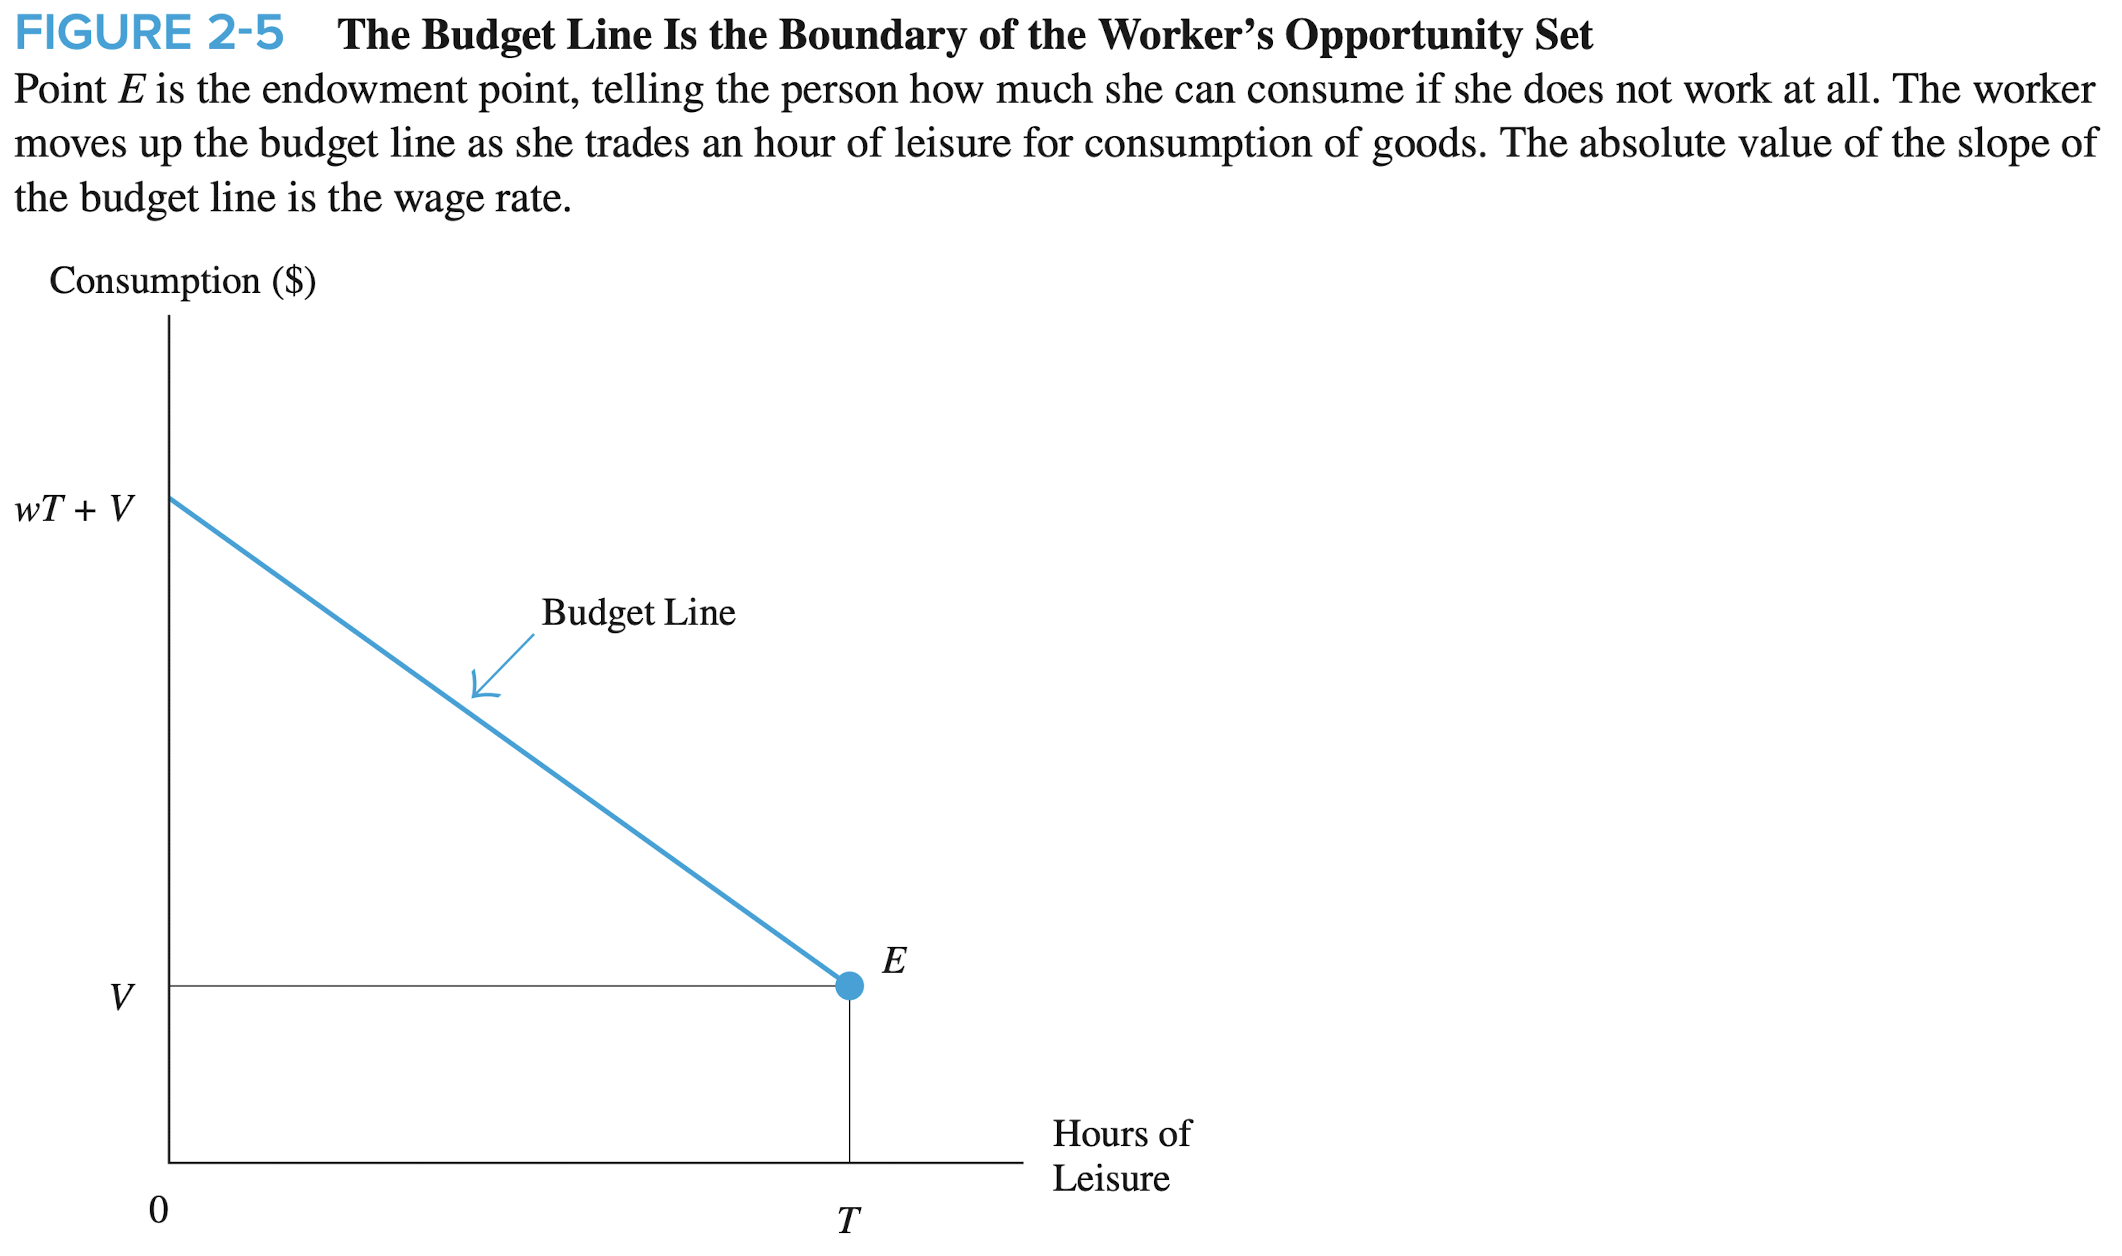
\includegraphics[width=0.9\textwidth]{../input/ch_2p4_oppor_set.png}
    \caption{Worker's Opportunity Set}
    \label{fig:ch2p4_oppor_set}
\end{figure}

\FloatBarrier

%%%%%%%%%%%%%%%%%%%%%%%%%%%%%%%%%%%%%%%%%%%%%%%%%%%%%%%%%%%%%%%%%%%%%%%%%%%%%%%%%%%%%%%
%%%%%%%%%%%%%%%%%%%%%%%%%%%%%%%%%%%%%%%%%%%%%%%%%%%%%%%%%%%%%%%%%%%%%%%%%%%%%%%%%%%%%%%
\subsection{The Hours of Work Decision}

Supposing there is an interior solution, i.e., the 
worker chooses to work some positive amount of hours but not all available hours,
the optimal choice of $C$ and $L$ occurs 
where the budget constraint is tangent to an indifference curve.
See \autoref{fig:ch2p5_tangency_cond} for an example.

\FloatBarrier

\begin{figure}[!htb]
    \centering
        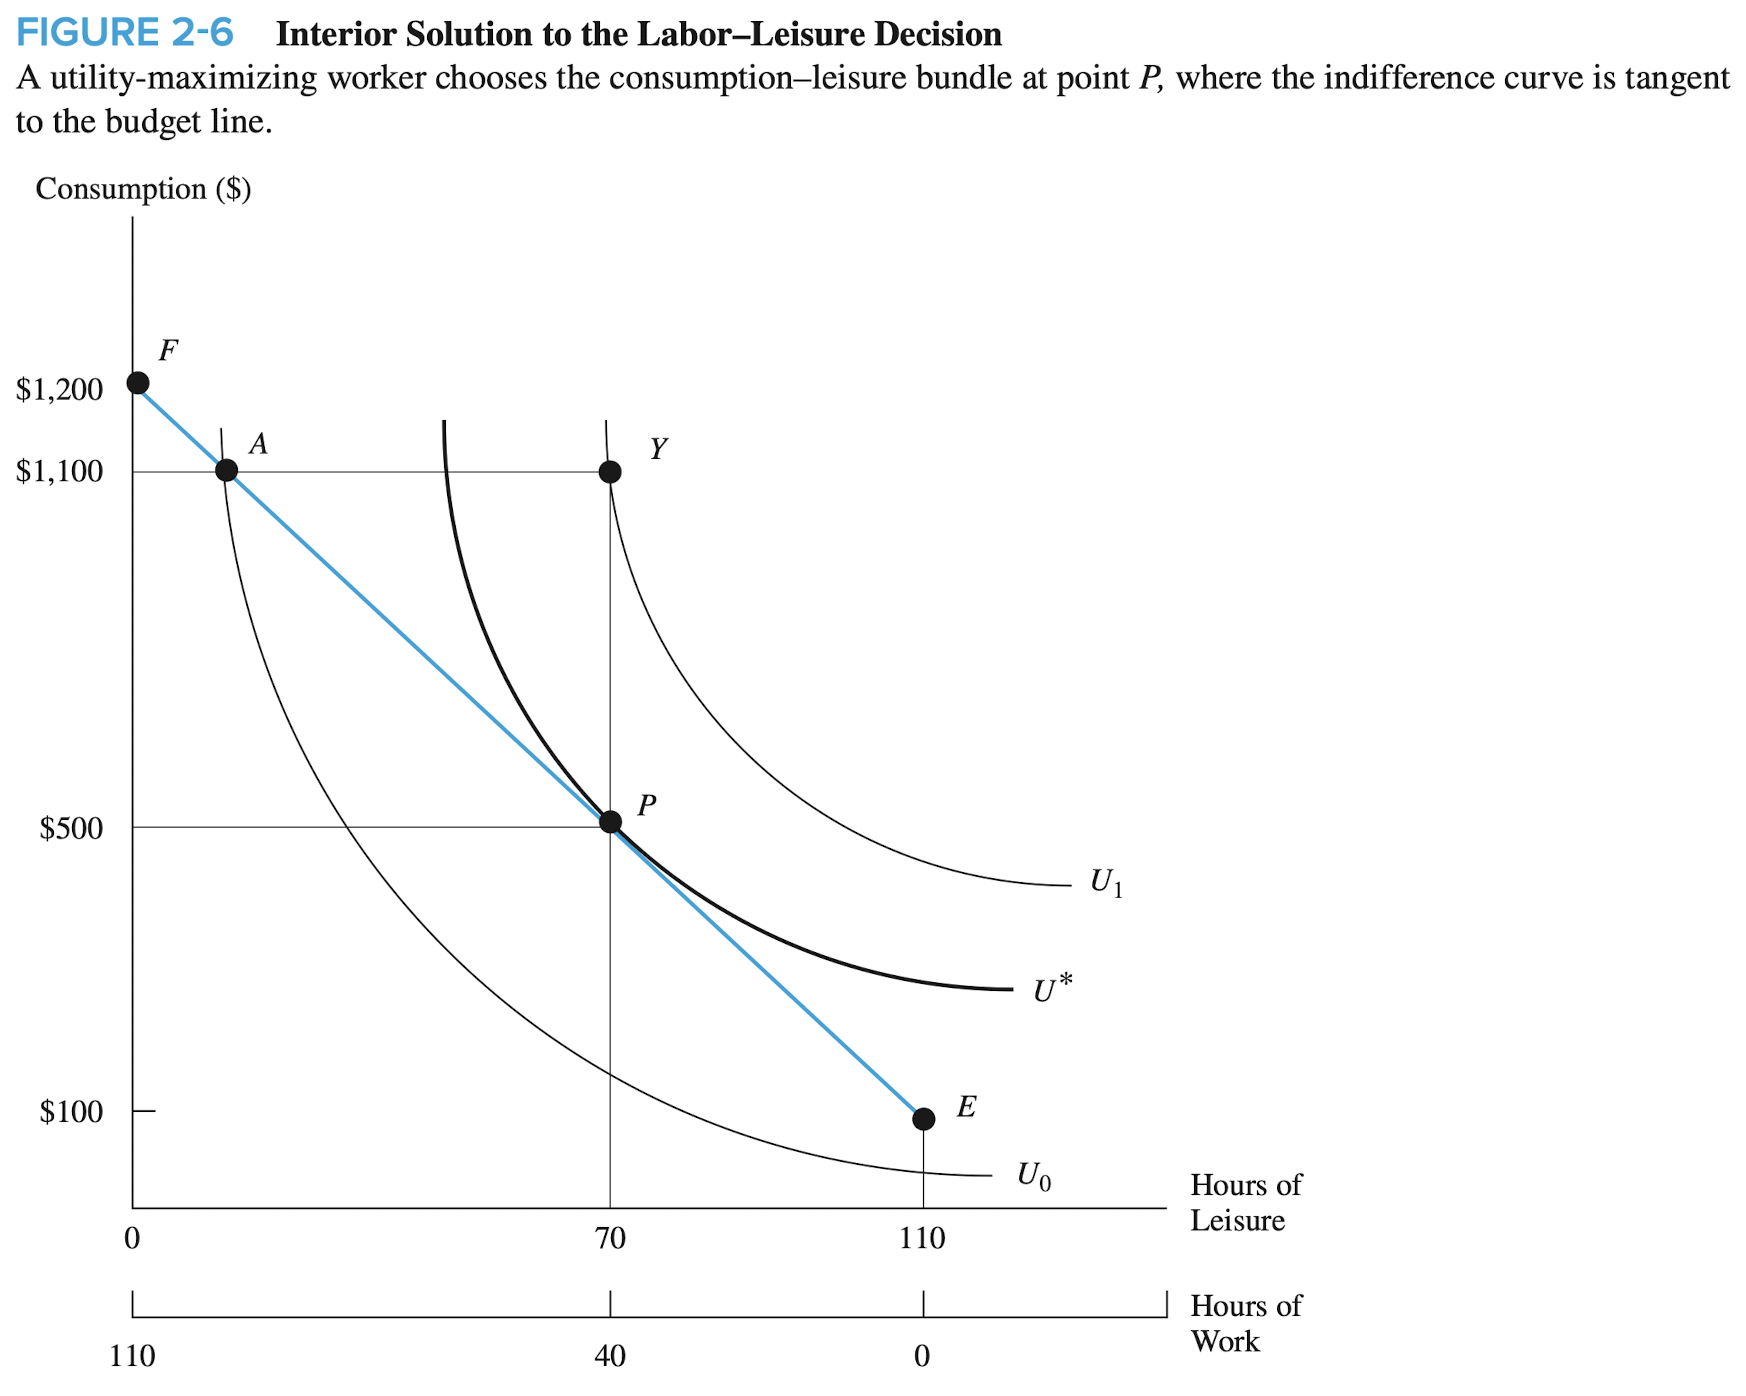
\includegraphics[width=0.9\textwidth]{../input/ch_2p5_tangency_cond.png}
    \caption{Tangency Condition for Optimal Choice}
    \label{fig:ch2p5_tangency_cond}
\end{figure}

\FloatBarrier

At the optimal point, denoted by $P$ 
in \autoref{fig:ch2p5_tangency_cond},
the slope of the indifference curve equals
the slope of the budget constraint.
That is,

\begin{align}
    \frac{MU_L}{MU_C} = w
\end{align}

This is easier to interpret, in my opinion, if 
we re-write it as:

\begin{align}
    MU_L = w MU_C
\end{align}

That is, we are indifferent between 
the marginal utility from an additional unit of 
leisure ($MU_L$) and the marginal 
utility from consumption ($MU_C$) multiplied by 
the amount of consumption that you could get
from working the extra hour ($w$).\footnote{I think
this is based on a normalization, so that 
the price of one unit of the consumption good 
is 1.} 
Thus, the last dollar spent on consumption
yields the same marginal utility as the last dollar
spent on leisure.

%%%%%%%%%%%%%%%%%%%%%%%%%%%%%%%%%%%%%%%%%%%%%%%%%%%%%%%%%%%%%%%%%%%%%%%%%%%%%%%%%%%%%%%
\subsubsection{What Happens to Hours of Work When Nonlabor Income Changes}

I won't spend long on this discussion, but see 
\autoref{fig:ch2p5_nonlabor_income_shock}
for a graphical depiction considering what happens
to consumption and leisure when nonlabor income ($V$) increases
and leisure is a normal or inferior good. 
Essentially this changes the frontier of the 
worker's opportunity set by shifting the intercept up 
without changing the slope.
Thus, it's a pure income effect, with no 
substitution effect.
If leisure is a normal good, which the author
suggests is probably the case, then this should 
lead to a decrease in hours worked.

\FloatBarrier

\begin{figure}[!htb]
    \centering
        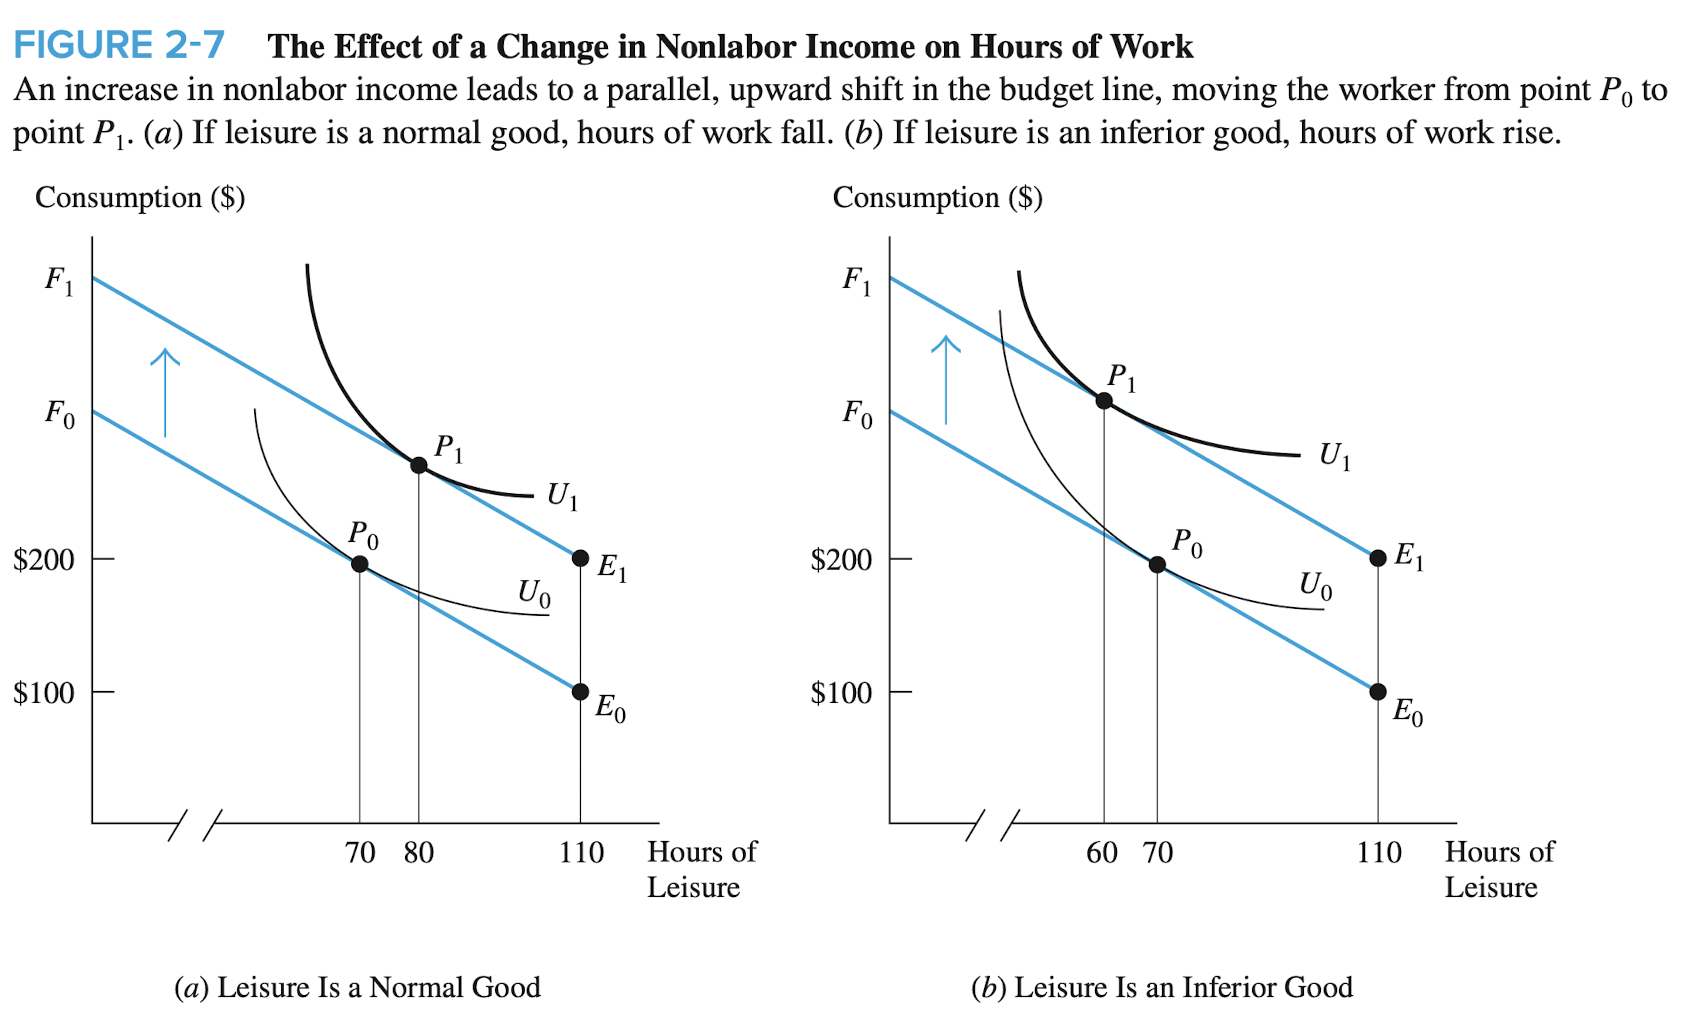
\includegraphics[width=0.9\textwidth]{../input/ch_2p5_nonlabor_income_shock.png}
    \caption{Effect of Nonlabor Income Shock on Hours of Work}
    \label{fig:ch2p5_nonlabor_income_shock}
\end{figure}

\FloatBarrier

%%%%%%%%%%%%%%%%%%%%%%%%%%%%%%%%%%%%%%%%%%%%%%%%%%%%%%%%%%%%%%%%%%%%%%%%%%%%%%%%%%%%%%%
\subsubsection{What Happens to Hours of Work When the Wage Changes?}

If there is a change to the worker's wage, then the effect
on hours worked is ambiguous, as we must contend 
with both income and substitution effects.
See \autoref{fig:ch2p5_wage_change}
for a graphic depiction of what happens to the 
worker's opportunity set when the wage increases,
as well as an example of indifference curves 
that could generate an increase or decrease in hours worked.

\FloatBarrier

\begin{figure}[!htb]
    \centering
        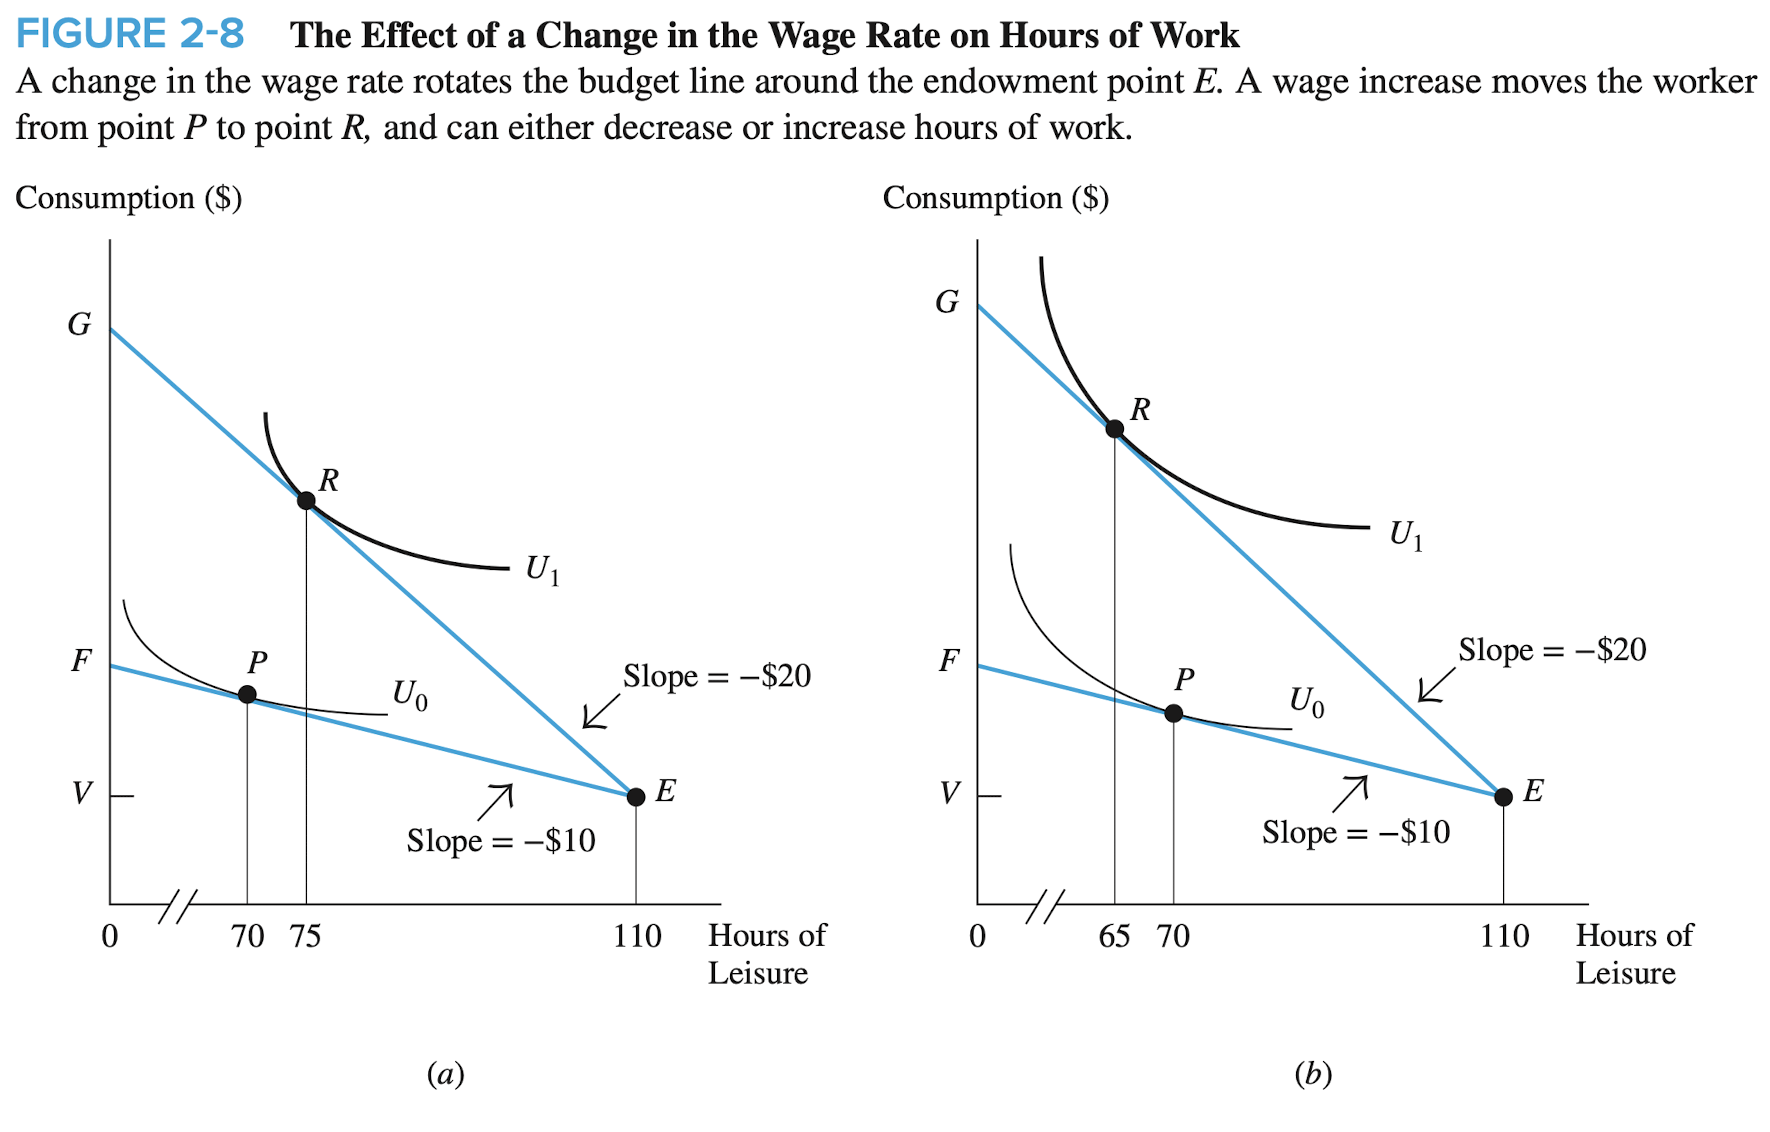
\includegraphics[width=0.9\textwidth]{../input/ch_2p5_wage_change.png}
    \caption{Effect of Wage Change on Hours of Work}
    \label{fig:ch2p5_wage_change}
\end{figure}

\FloatBarrier

\autoref{fig:ch2p5_effect_decomp} decomposes the 
effect of the wage change into the income and substitution effects.
In this decomposition, the pre-wage-change level of 
consumption and leisure is given by $P$.
After the wage change, the move from $P$ 
to $Q$ is the income effect, in which the worker 
works fewer hours due to the increase in income. We 
visualize this with a parallel shift in the budget constraint,\footnote{When I say 
budget constraint here, I guess I really mean the opportunity set frontier.}
as we did in \autoref{fig:ch2p5_nonlabor_income_shock} when the 
worker experienced a non-wage income shock. The income effect portion is 
thus characterized by a change in the
intercept of the budget constraint line, but not the slope.

The substitution effect is then the move from $Q$ to $R$,
in which the worker works more hours due to the
increase in the wage. In contrast to when the worker 
experienced a non-wage income shock, leisure has now become 
more expensive, in the sense that the opportunity cost of
leisure has increased. The substitution effect can be thought of 
as what happens to the worker's choice of $C$ and $L$
as the wage changes but the worker's level of utility is held constant,
in this case at the level associated with $U_1$.

As demonstrated in \autoref{fig:ch2p5_effect_decomp}, 
the overall effect of the wage change on hours worked
is ambiguous, as it depends on the relative magnitudes
of the income and substitution effects.

\FloatBarrier

\begin{figure}[!htb]
    \centering
        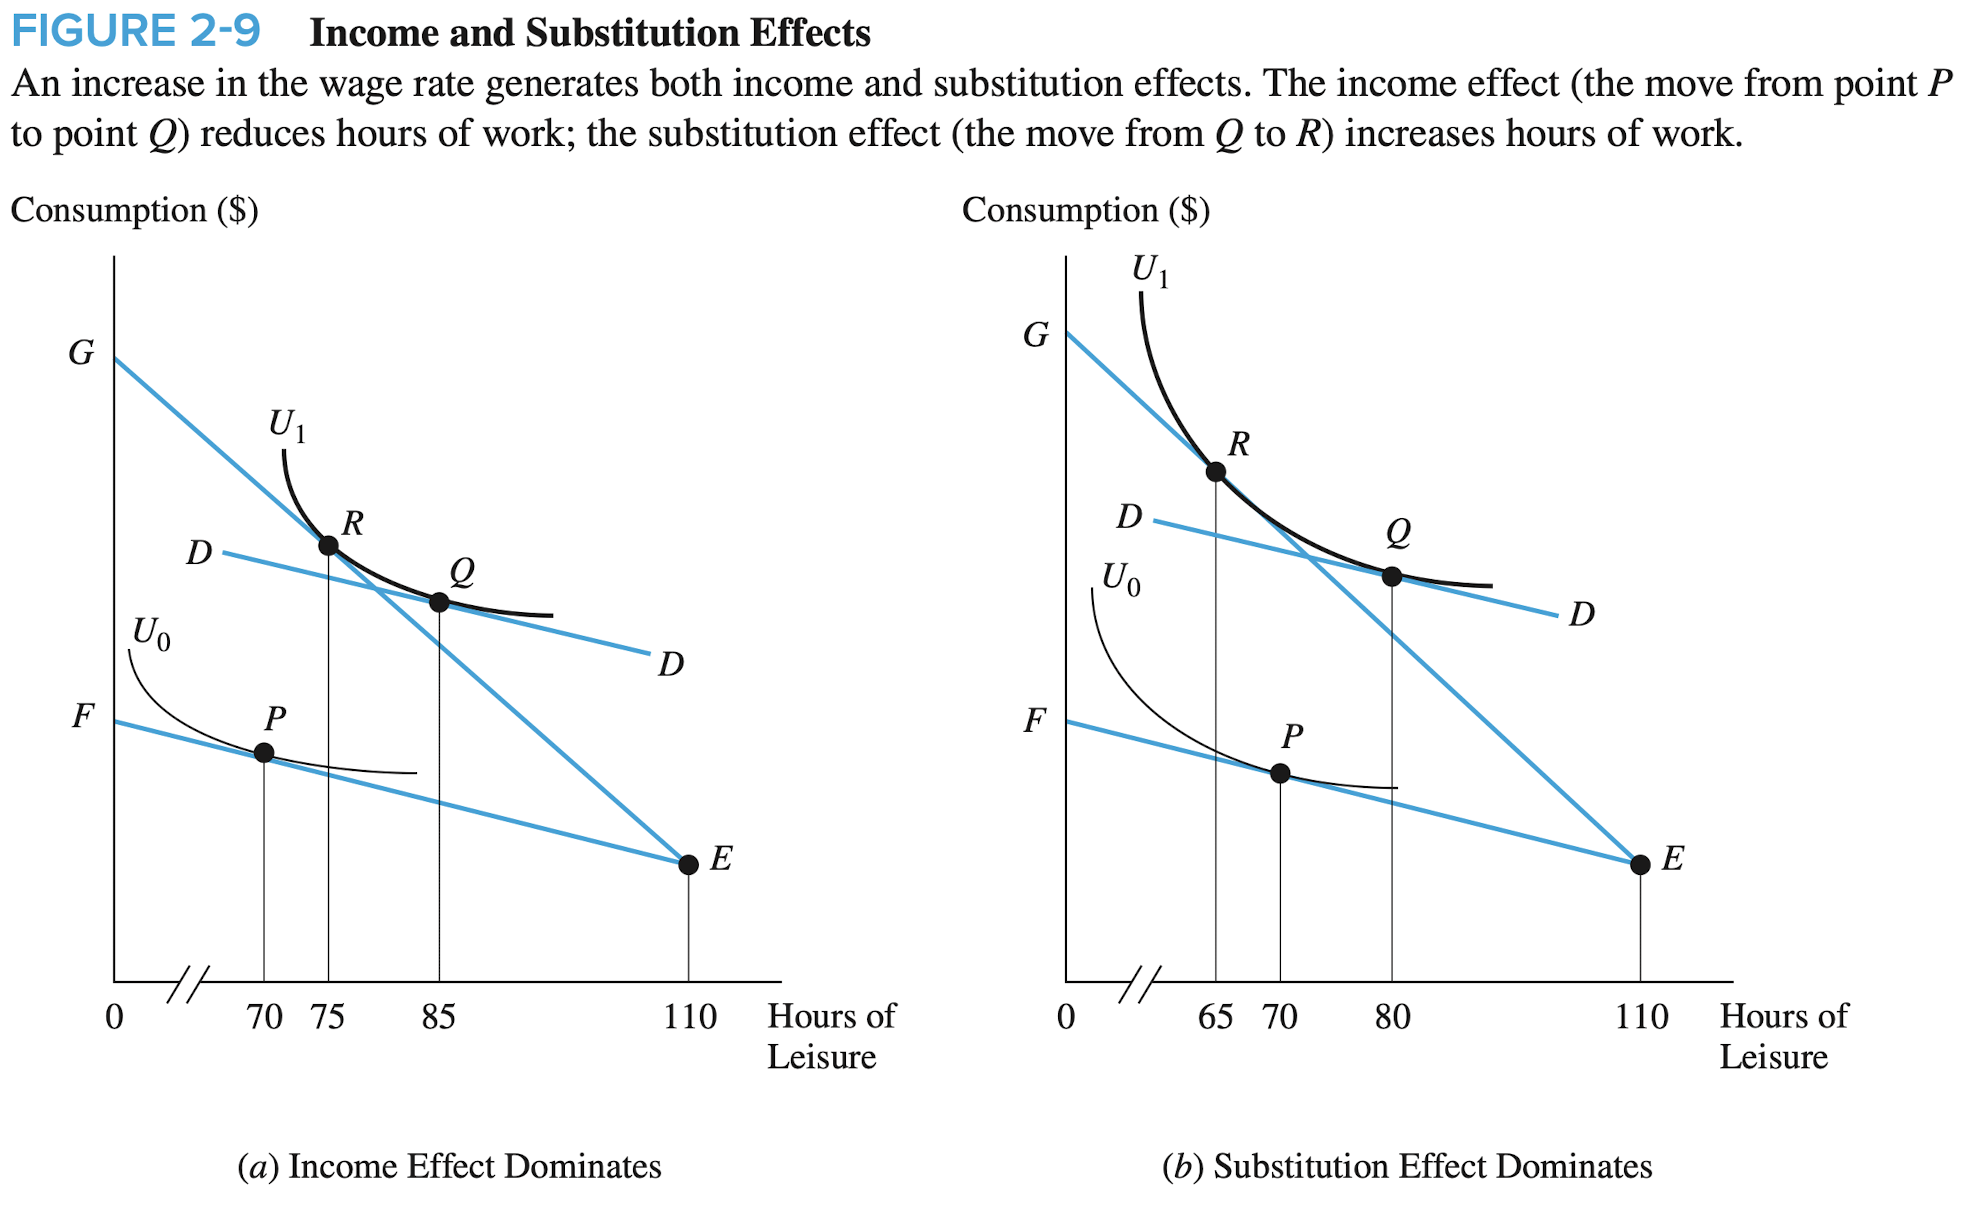
\includegraphics[width=0.9\textwidth]{../input/ch_2p5_effect_decomp.png}
    \caption{Decomposition of Wage Change Effects}
    \label{fig:ch2p5_effect_decomp}
\end{figure}

\FloatBarrier

%%%%%%%%%%%%%%%%%%%%%%%%%%%%%%%%%%%%%%%%%%%%%%%%%%%%%%%%%%%%%%%%%%%%%%%%%%%%%%%%%%%%%%%
%%%%%%%%%%%%%%%%%%%%%%%%%%%%%%%%%%%%%%%%%%%%%%%%%%%%%%%%%%%%%%%%%%%%%%%%%%%%%%%%%%%%%%%
\subsection{To Work or Not to Work?}

A worker may choose not to work at all.
Look at \autoref{fig:ch2p6_work_dec} for an example.
At wage $w_{\text{low}}$, the worker chooses not to work.
This is because the utility curve that they're on
at their initial endowment point $E$ ($U_0$) is higher 
than any utility curve that they could reach along the 
line $GE$ characterizing their opportunity set
under wage $w_{\text{low}}$.
However, if the wage increases to $w_{\text{high}}$,
then, they could reach point $Y$ on indifference curve $U_H$, 
which is higher than $U_0$. Thus, they work at wage $w_{\text{high}}$.
In fact, we can pinpoint the exact point at which 
the worker is indifferent between working and not working.
This occurs at the wage $w^*$, which is the 
absolute value of the slope of the line tangent to
the indifference curve $U_0$ at point $E$.
We refer to this as the reservation wage.

\begin{definition}[Reservation Wage]

    The reservation wage is the wage at which the worker is 
    indifferent between working and not working.
    
\end{definition}

Note that the probability of working is increasing in the wage -- 
only the substitution effect applies, since the income effect of 
a wage increase doesn't kick in if the person wasn't working to begin with.

\FloatBarrier

\begin{figure}[!htb]
    \centering
        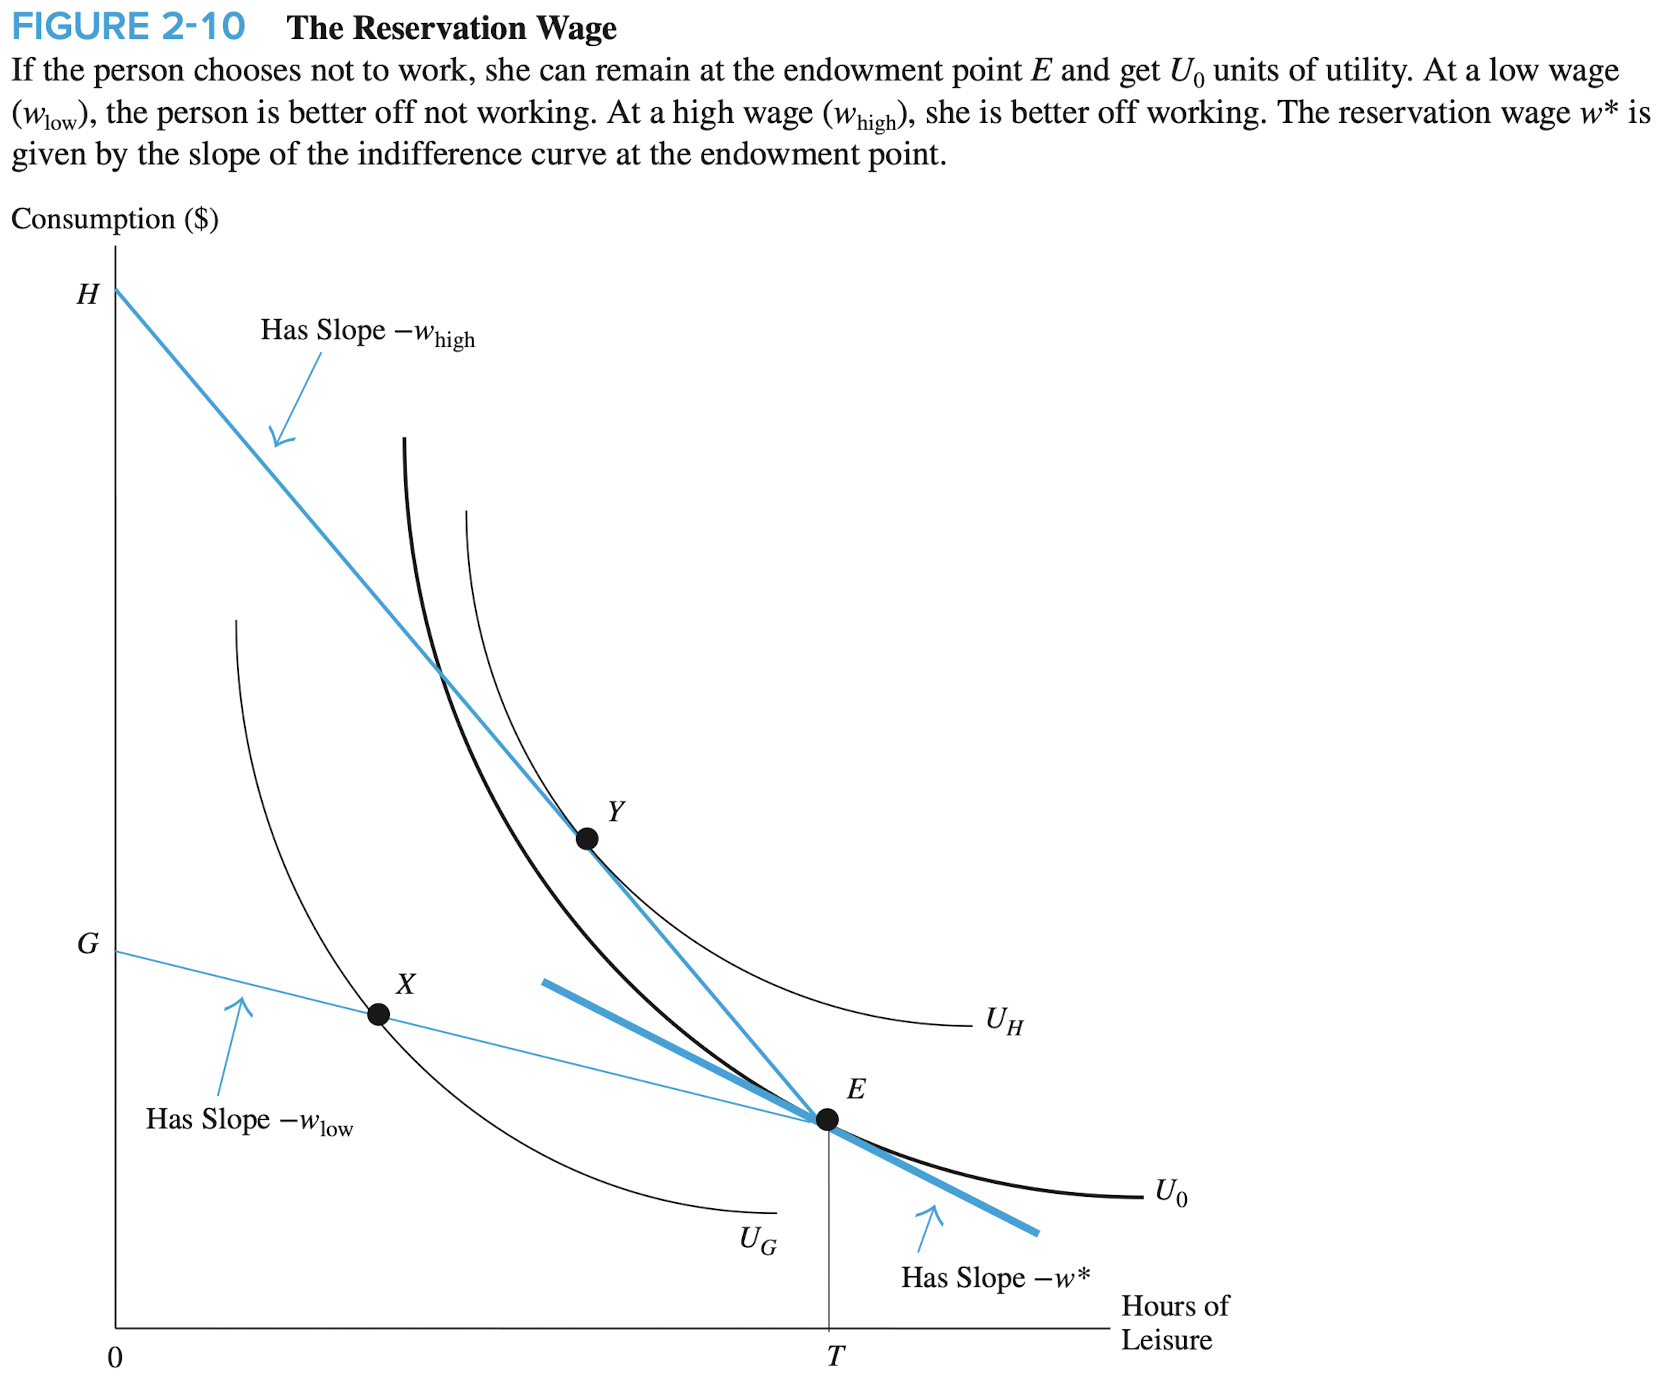
\includegraphics[width=0.9\textwidth]{../input/ch_2p6_work_dec.png}
    \caption{Decision to Work}
    \label{fig:ch2p6_work_dec}
\end{figure}

\FloatBarrier

%%%%%%%%%%%%%%%%%%%%%%%%%%%%%%%%%%%%%%%%%%%%%%%%%%%%%%%%%%%%%%%%%%%%%%%%%%%%%%%%%%%%%%%
%%%%%%%%%%%%%%%%%%%%%%%%%%%%%%%%%%%%%%%%%%%%%%%%%%%%%%%%%%%%%%%%%%%%%%%%%%%%%%%%%%%%%%%
\subsection{The Labor Supply Curve}

There is a tight relationship between the 
utility maximization problem that we've been 
discussing and the worker's labor supply 
curve. 
Indeed, the latter can be derived from the former,
as demonstrated in \autoref{fig:ch2p7_derive_labor_supply}.
At each wage, the worker chooses a level of 
hours to spend on leisure ($L$), the hours worked is 
then $h = T - L$, where $T$ is the total hours available.
Thus, for each wage, we have the worker's corresponding 
number of hours of labor supplied, which is what we need 
to plot the labor supply curve. 
In the example we consider in 
\autoref{fig:ch2p7_derive_labor_supply}, 
the substitution effect dominates up until 
the wage hits $20$, after which point, the income 
effect dominates and the number of hours worked 
declines.

\FloatBarrier

\begin{figure}[!htb]
    \centering
        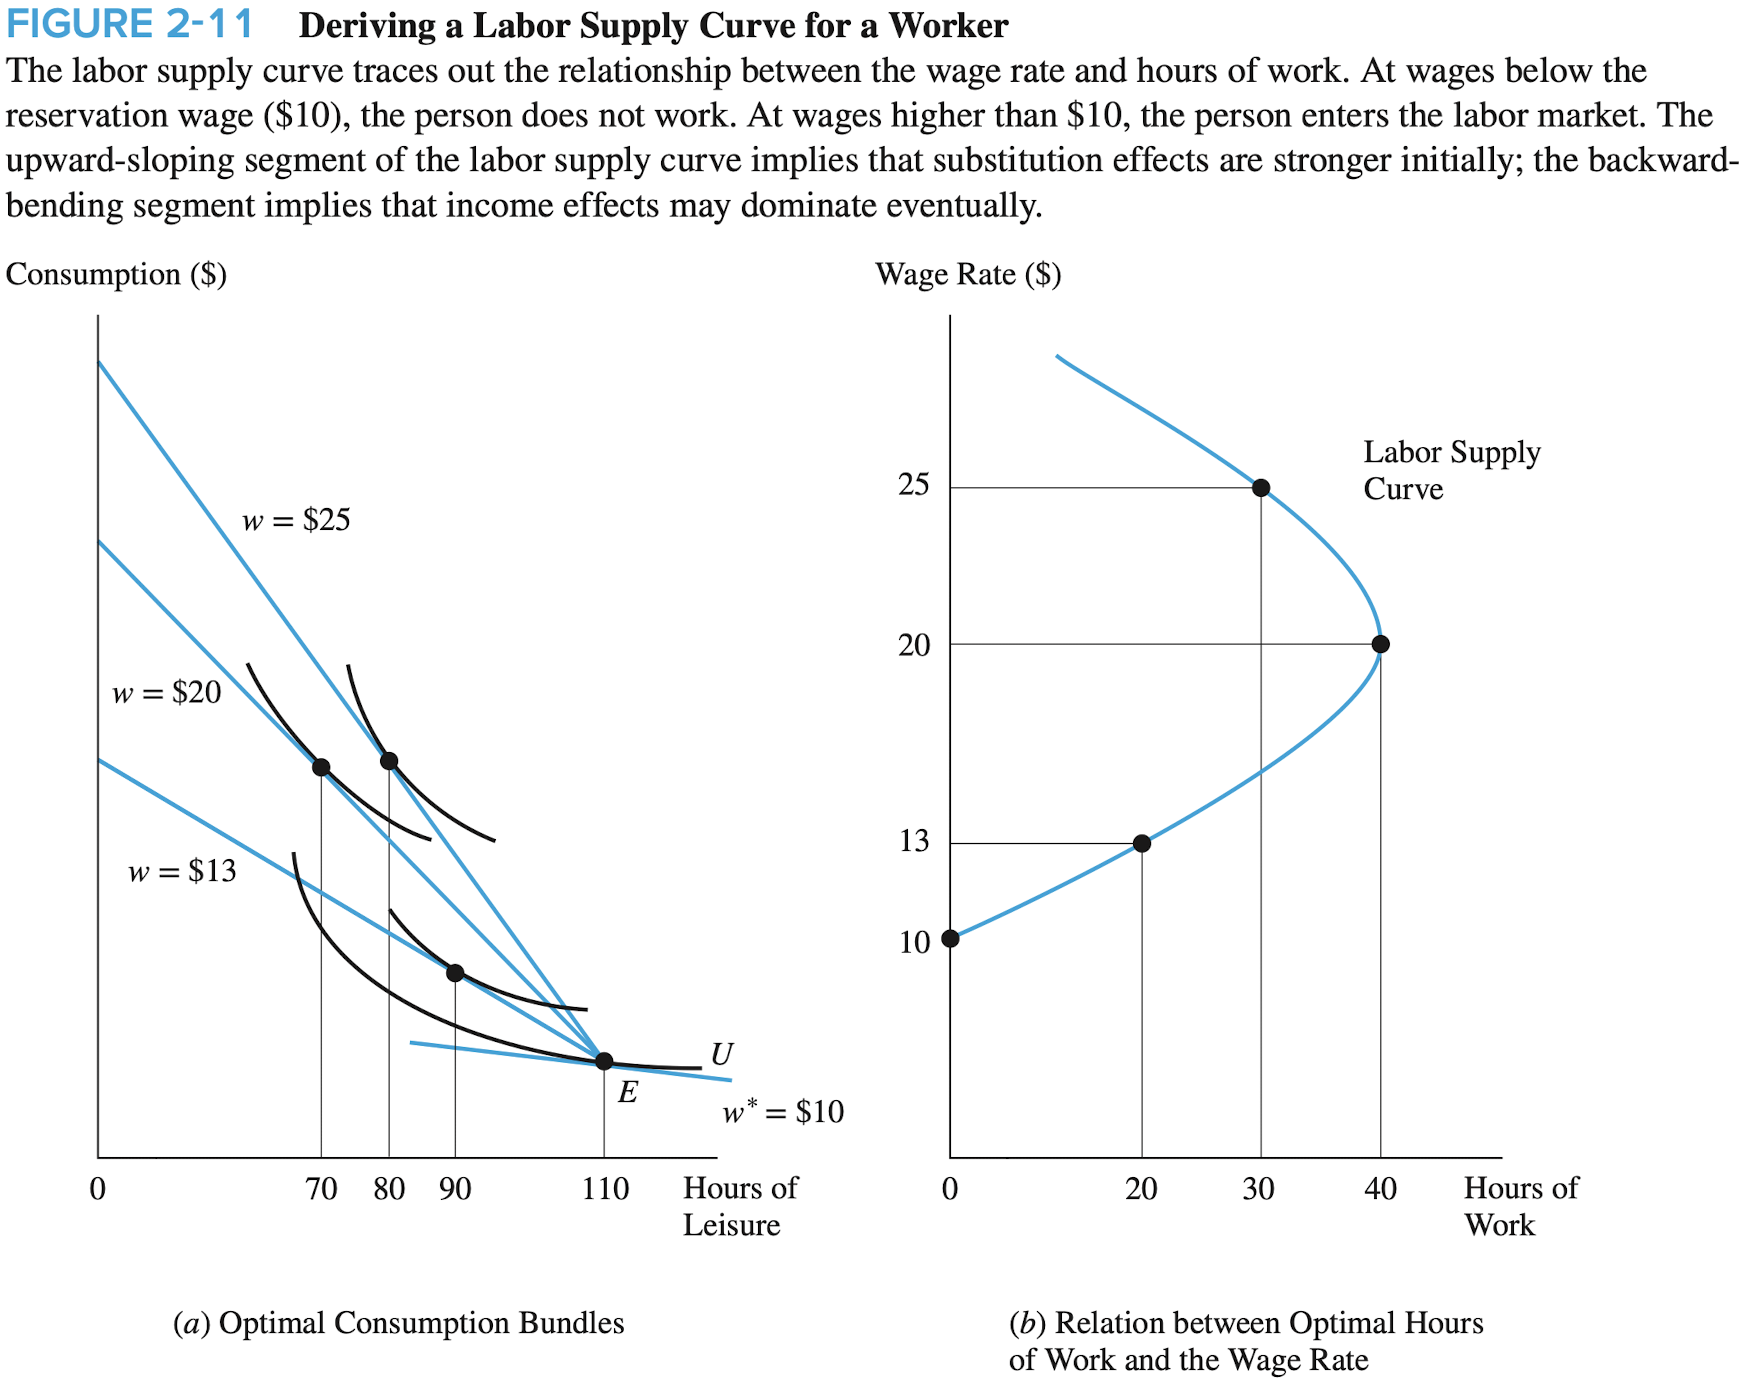
\includegraphics[width=0.9\textwidth]{../input/ch_2p7_derive_labor_supply.png}
    \caption{Derivation of the Labor Supply Curve}
    \label{fig:ch2p7_derive_labor_supply}
\end{figure}

\FloatBarrier

The aggregate labor supply is the sum of the 
individual labor supply decisions. 
See \autoref{fig:ch2p7_agg_labor_supply} for an example
with two workers.

\FloatBarrier

\begin{figure}[!htb]
    \centering
        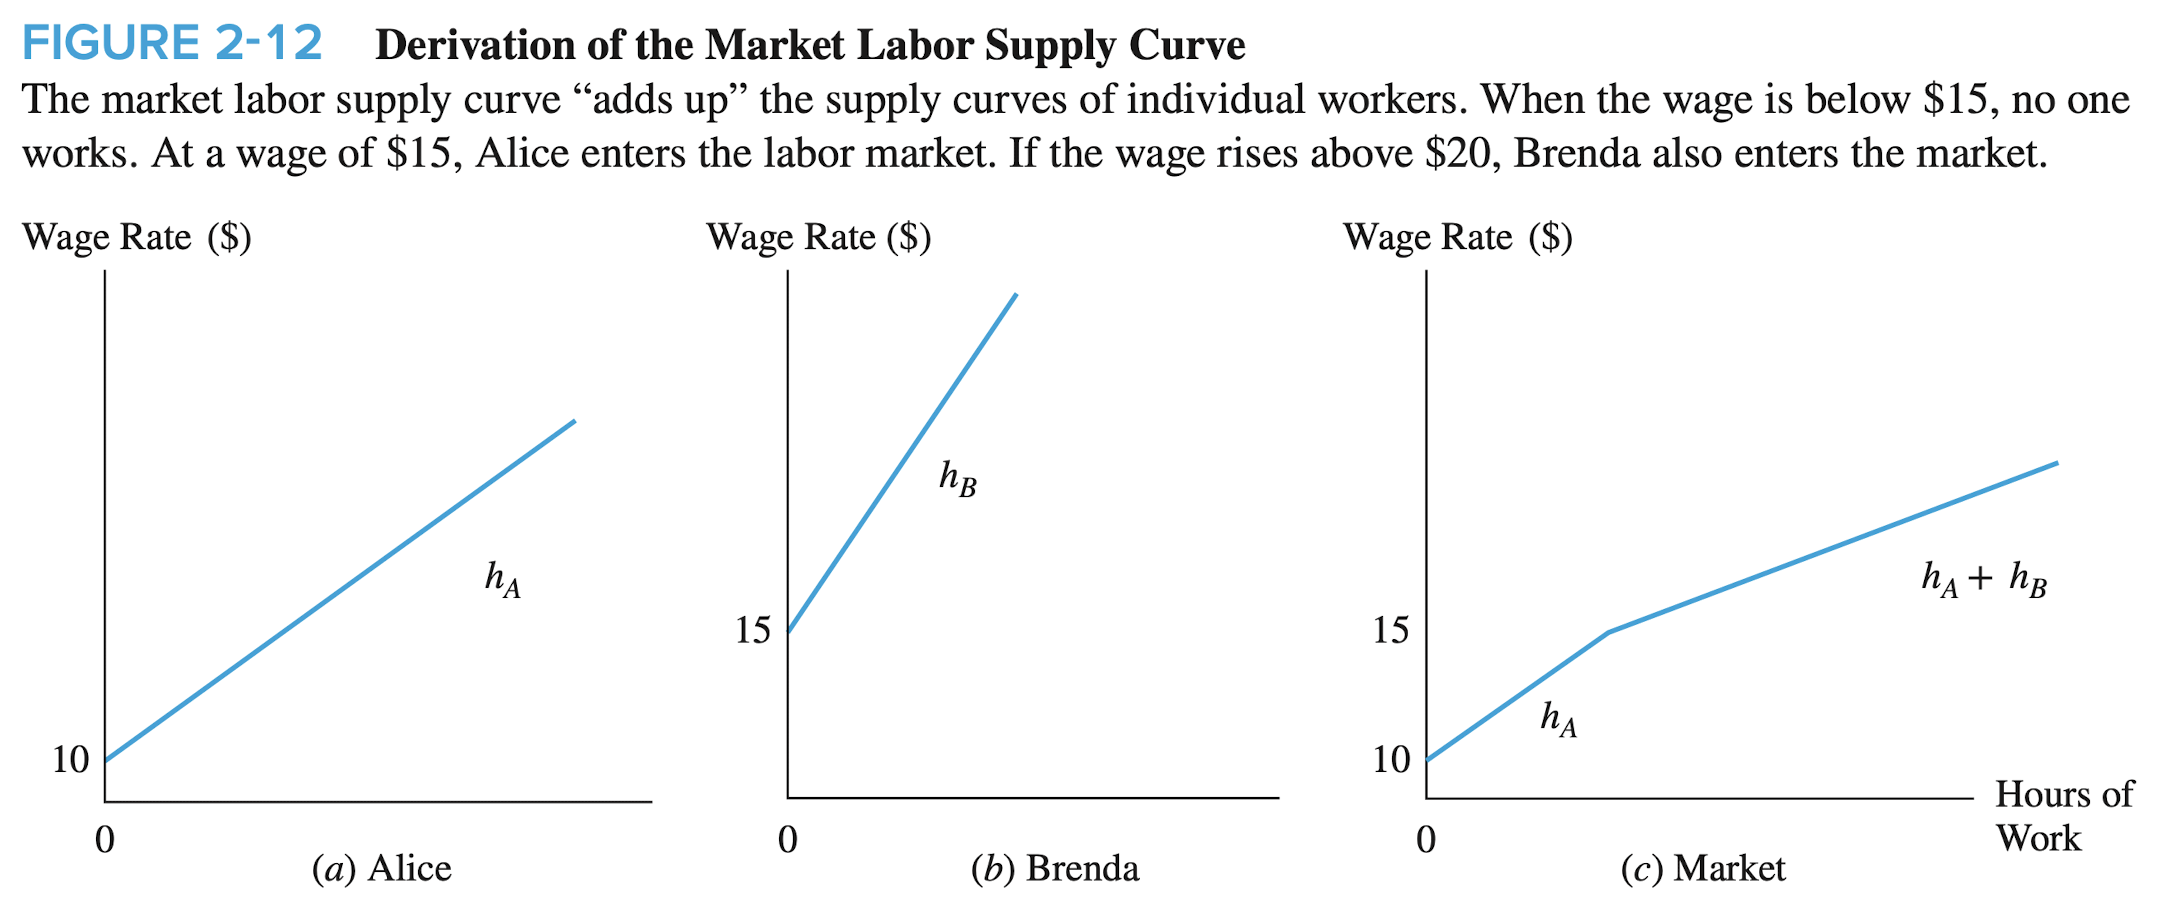
\includegraphics[width=0.9\textwidth]{../input/ch_2p7_agg_labor_supply.png}
    \caption{Aggregate Labor Supply}
    \label{fig:ch2p7_agg_labor_supply}
\end{figure}

\FloatBarrier

We then consider the notion of labor supply elasticity.
Labor supply elasticity tells us what percent change in 
hours worked corresponds to a percent change in the wage.

\begin{definition}[Labor Supply Elasticity] 

    The labor supply elasticity is 
    a measure of how responsive hours worked ($h$) 
    is to changes in the wage ($w$). 
    It is given by the expression for $\sigma$ below.
    
    \begin{align}
        \sigma= \underbrace{\left(\frac{\Delta h}{h}\right)}_{\parbox[t]{2cm}{\raggedright \footnotesize \centering Percent change in hours worked}} / \underbrace{\left(\frac{\Delta w}{w}\right)}_{\parbox[t]{2cm}{\raggedright \footnotesize \centering Percent change in wage}} =\frac{\Delta h}{\Delta w} \cdot \frac{w}{h}
    \end{align}

\end{definition}

\begin{definition}[Elastic and Inelastic] 
    
    If $\sigma > 1$, then labor supply is elastic.
    If $\sigma < 1$, then labor supply is inelastic.
    If $\sigma = 1$, then labor supply has unit elasticity.

\end{definition}

%%%%%%%%%%%%%%%%%%%%%%%%%%%%%%%%%%%%%%%%%%%%%%%%%%%%%%%%%%%%%%%%%%%%%%%%%%%%%%%%%%%%%%%
%%%%%%%%%%%%%%%%%%%%%%%%%%%%%%%%%%%%%%%%%%%%%%%%%%%%%%%%%%%%%%%%%%%%%%%%%%%%%%%%%%%%%%%
\subsection{Estimates of the Labor Supply Elasticity}

Some evidence suggests that the labor supply elasticity
for men is around $-0.1$. That is, the income effect is 
dominating for men, which could explain the decline in hours 
worked among men over the last century, as real wages have increased.
However, there are meaningful challenges in estimating the
labor supply elasticity, e.g.,
measurement error. 

%%%%%%%%%%%%%%%%%%%%%%%%%%%%%%%%%%%%%%%%%%%%%%%%%%%%%%%%%%%%%%%%%%%%%%%%%%%%%%%%%%%%%%%
%%%%%%%%%%%%%%%%%%%%%%%%%%%%%%%%%%%%%%%%%%%%%%%%%%%%%%%%%%%%%%%%%%%%%%%%%%%%%%%%%%%%%%%
\subsection{Household Production}

The neoclassical model of labor-leisure choice
is built on the idea that we can either engage in 
leisure or wage labor. However, we often 
engage in home production, in which we 
produce goods and services for our own consumption.
We now incorporate this into a model of labor supply
that considers a household (in this case, 2 workers), 
rather than just an individual.

%%%%%%%%%%%%%%%%%%%%%%%%%%%%%%%%%%%%%%%%%%%%%%%%%%%%%%%%%%%%%%%%%%%%%%%%%%%%%%%%%%%%%%%

\subsubsection{The Household Production Function}

\begin{definition}[The Household Production Function] 
    
    The household production function describes the level of household 
    output producible by the household for a given amount of time.

\end{definition}

See \autoref{fig:ch2p10_hh_prod} for an example.
In this example, we consider a couple, Jack and Jill.
Panels (a) and (b) show the opportunity sets for 
Jack and Jill individually, respectively.
Panel (c) shows the household production function,
which is derived from the individual opportunity sets.
In this scenario, we suppose that Jack can earn more
in the market and produce less in the household 
per hour. Thus, the slope of the household opportunity 
frontier varies as it switches from the marginal 
productivity coming from Jack to Jill or vice versa.

One of the key implications of this model 
is that each member of the household should 
be prioritized for the activity in which they are 
comparatively better. For example, if the couple needs 
to move from a world in which they engage exclusively in 
home production to one in which some hours of work 
are allocated to the market, this model would prioritize 
Jack working in the market, since he has the higher
wage and lower household productivity.


\FloatBarrier

\begin{figure}[!htb]
    \centering
        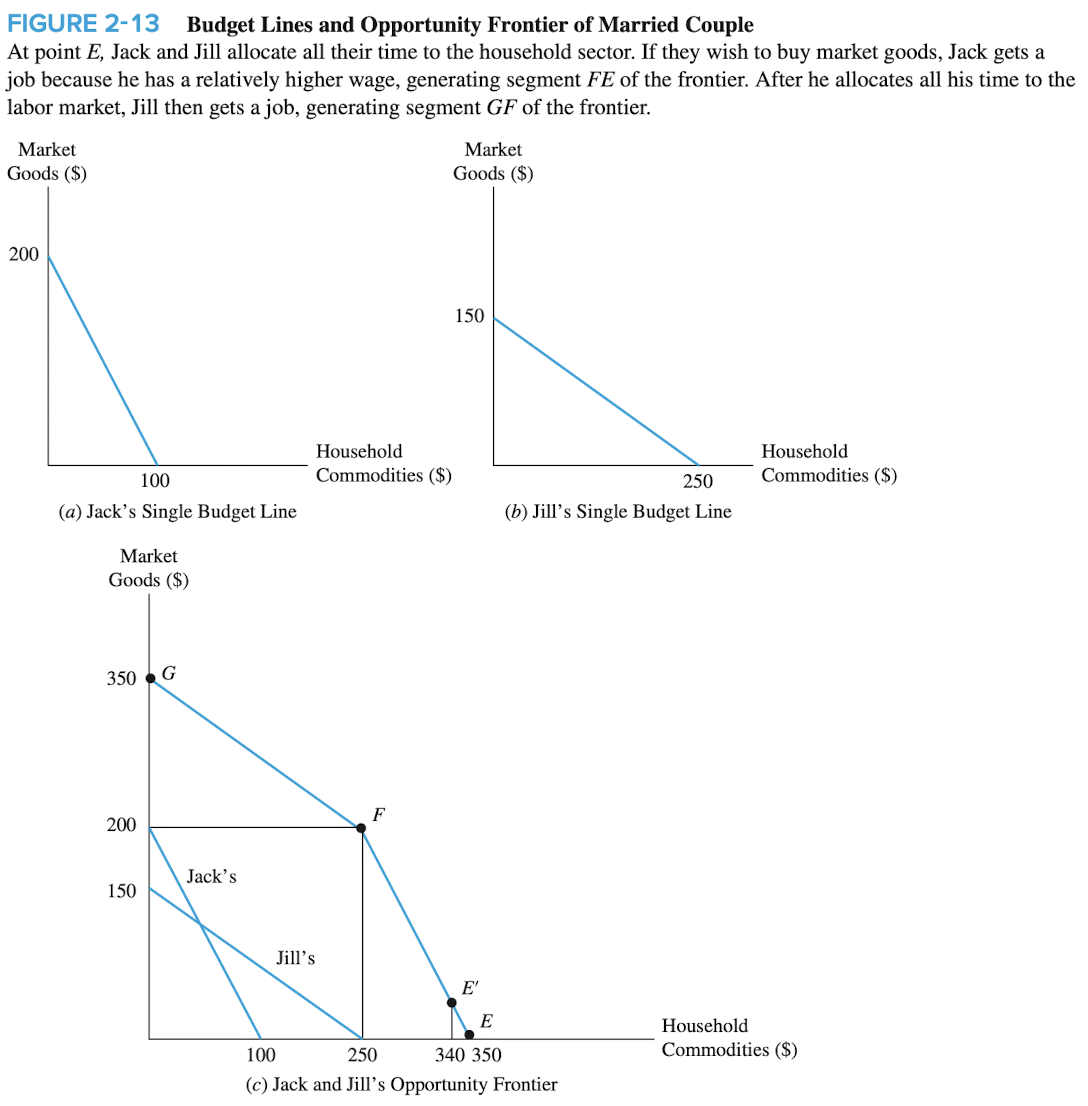
\includegraphics[width=0.95\textwidth]{../input/ch_2p10_hh_prod.png}
    \caption{Household Production Function}
    \label{fig:ch2p10_hh_prod}
\end{figure}

\FloatBarrier

\autoref{fig:ch2p10_hh_utils} shows various 
possible allocations of Jack and Jill's
time between market work and home production that 
might be justified under different 
utility functions.

\FloatBarrier

\begin{figure}[!htb]
    \centering
        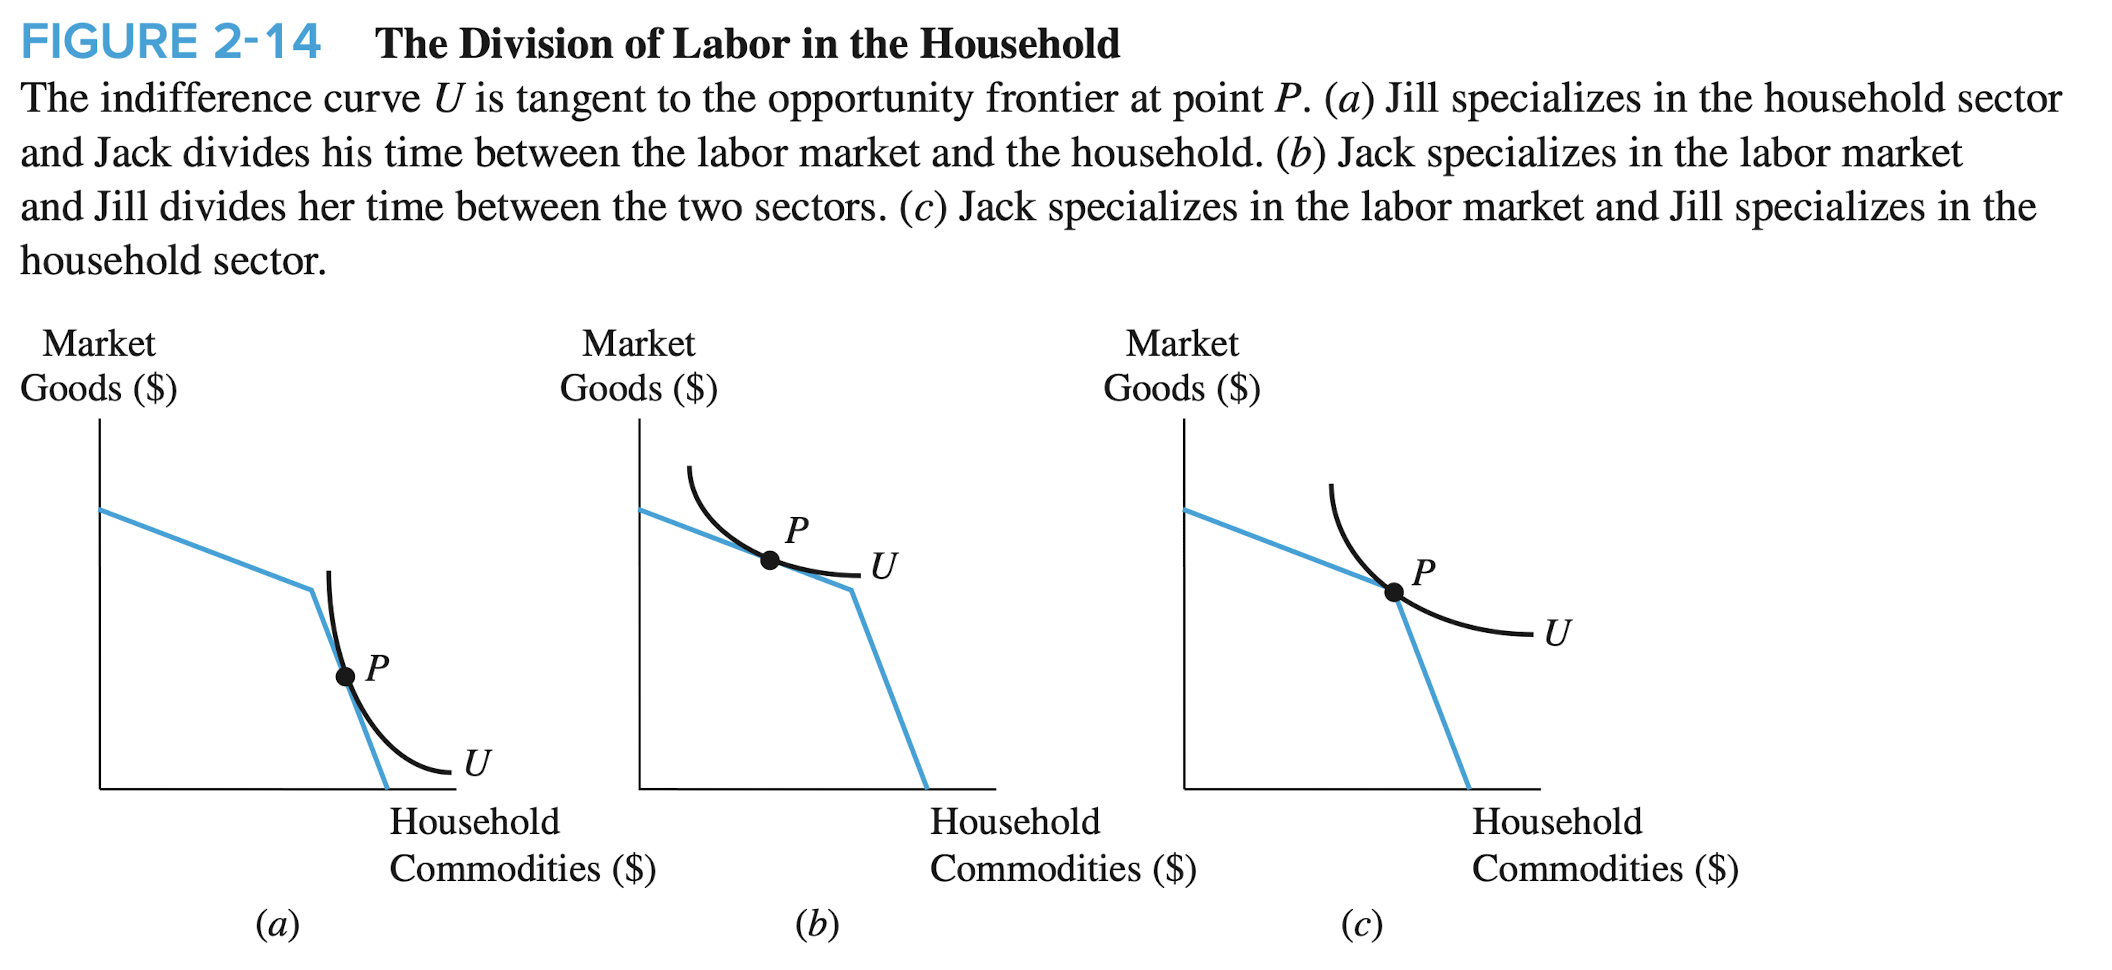
\includegraphics[width=0.95\textwidth]{../input/ch_2p10_hh_utils.png}
    \caption{Various Household Allocations}
    \label{fig:ch2p10_hh_utils}
\end{figure}

\FloatBarrier

\autoref{fig:ch2p10_hh_wage_change}
captures what happens if Jack experiences an increase 
in wage or Jill experiences an increase in
household productivity.
In the first case, Jack shifts away from home 
production towards market work.
In the second case, Jill shifts away from market work
towards home production. In each case, these particular figures 
show complete specialization. In Panel (a), I show
an extra bullet if there was no change in Jack's 
allocation between market work and home production.
At this point, we can see that the household would only have to 
give up a little bit of household commodity
to get much more in market goods, because of the 
newfound steepness of this portion of the household production frontier.

\begin{figure}[!htb]
    \centering
        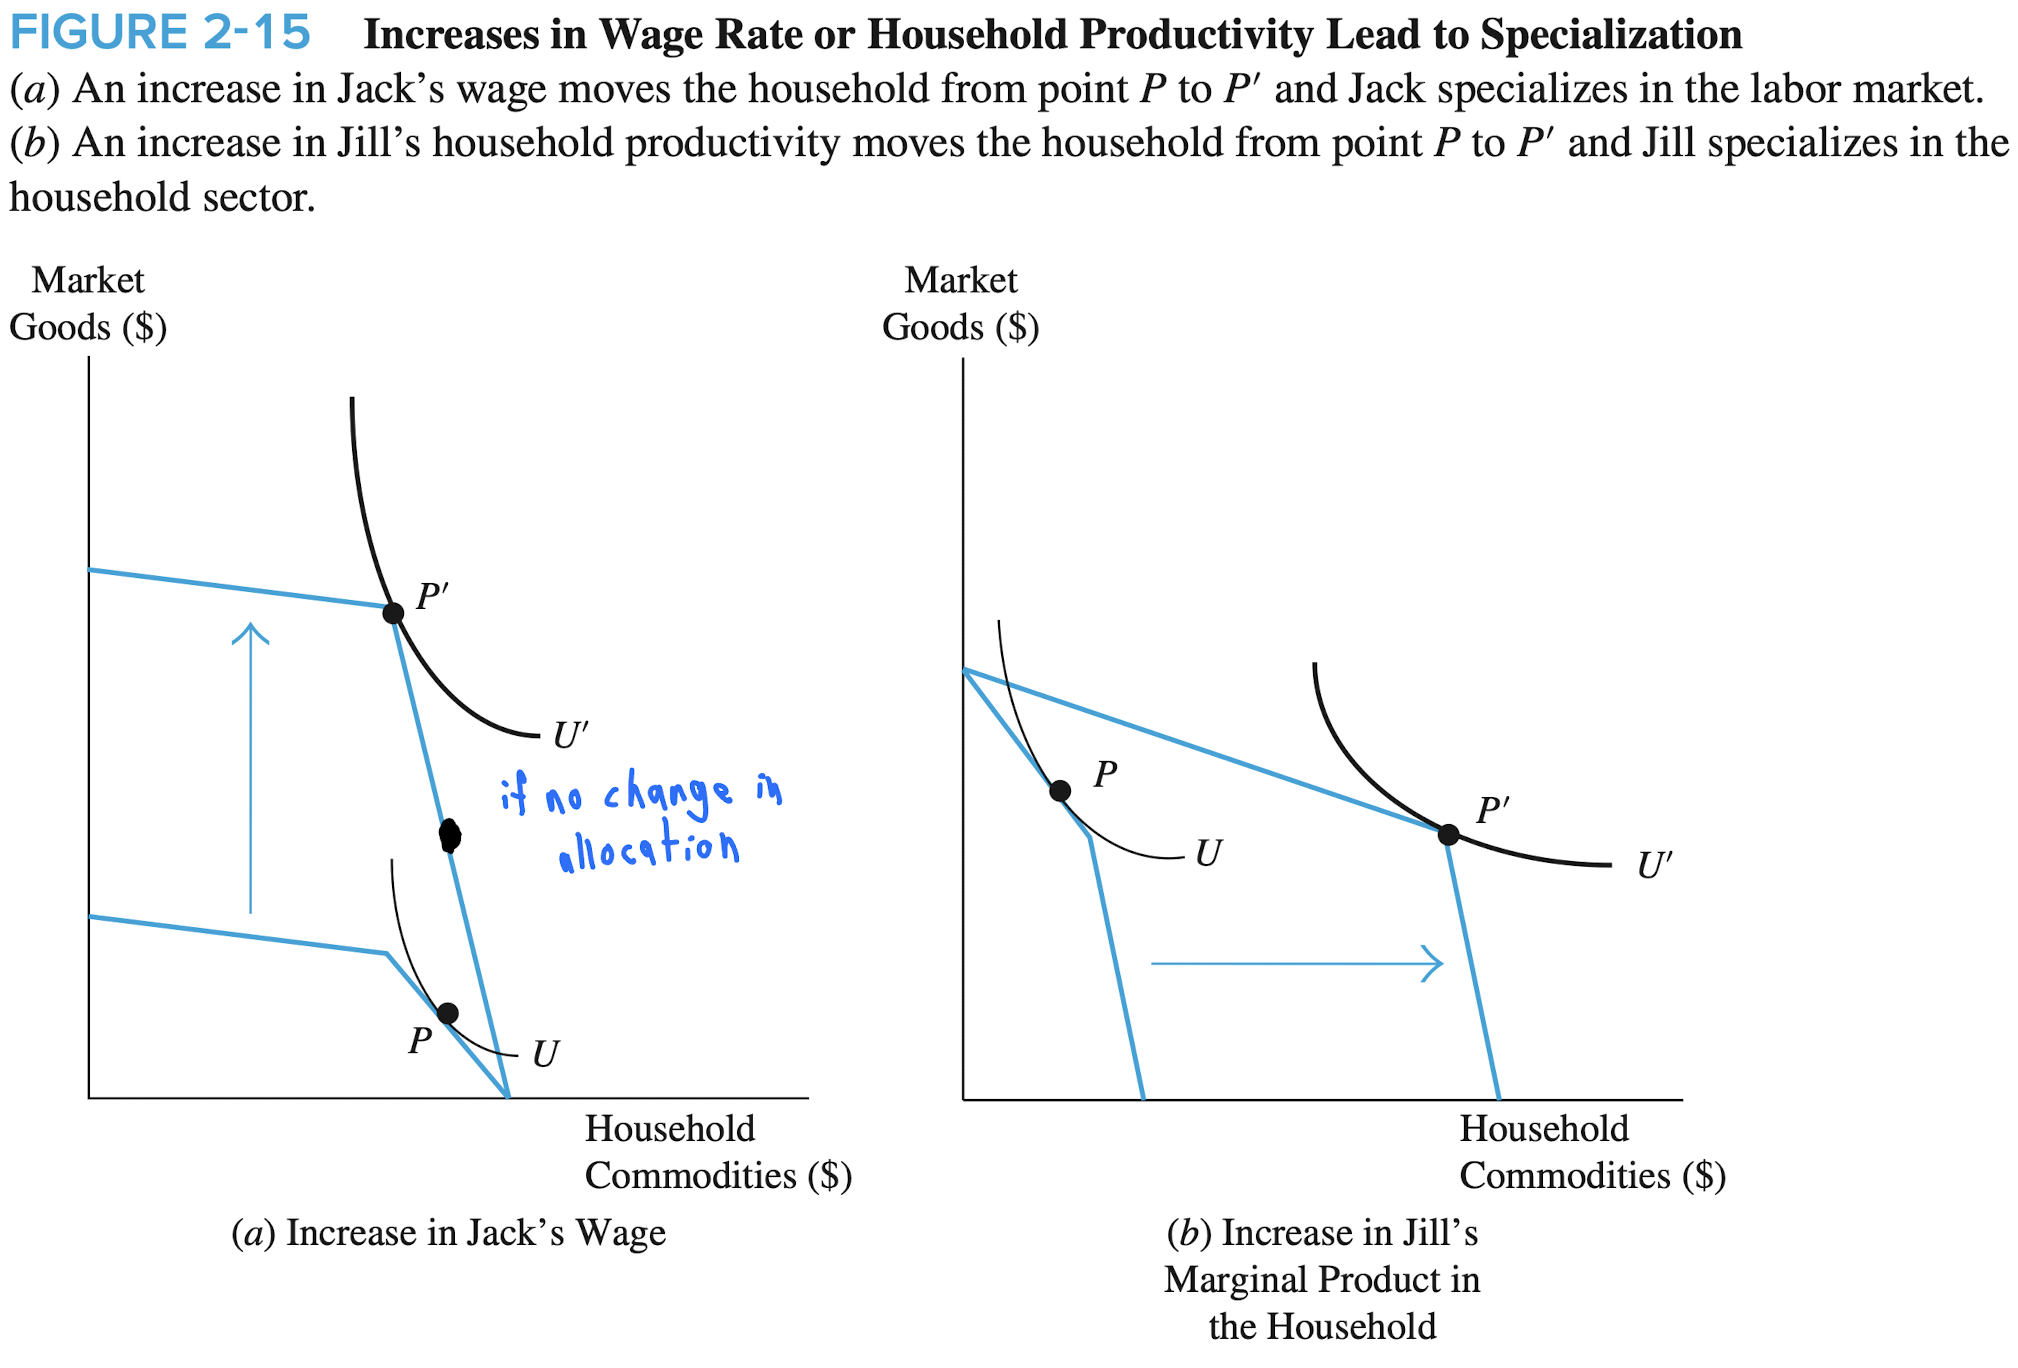
\includegraphics[width=0.9\textwidth]{../input/ch_2p10_hh_wage_change.png}
    \caption{Impact of Wage or HH Production Changes on Household Production}
    \label{fig:ch2p10_hh_wage_change}
\end{figure}

%%%%%%%%%%%%%%%%%%%%%%%%%%%%%%%%%%%%%%%%%%%%%%%%%%%%%%%%%%%%%%%%%%%%%%%%%%%%%%%%%%%%%%%
%%%%%%%%%%%%%%%%%%%%%%%%%%%%%%%%%%%%%%%%%%%%%%%%%%%%%%%%%%%%%%%%%%%%%%%%%%%%%%%%%%%%%%%
\subsection{Policy Application: Welfare Programs and Work Incentives}

This section considers the impact of various forms of welfare on 
work incentives. 
First, \autoref{fig:ch2p11_cash_grant}
shows how a cash grant to those working zero hours 
could reduce a worker's supply of labor. 
In this figure, we see that the worker supplies $G$ 
hours of labor at the considered wage, but if they receive
$1,000$ for not working, they reach a higher indifference curve 
by taking the grant and not working at all. Thus, the
worker with these example indifference curves facing this
binary grant would choose not to work when they otherwise would've.

\FloatBarrier

\begin{figure}[!htb]
    \centering
        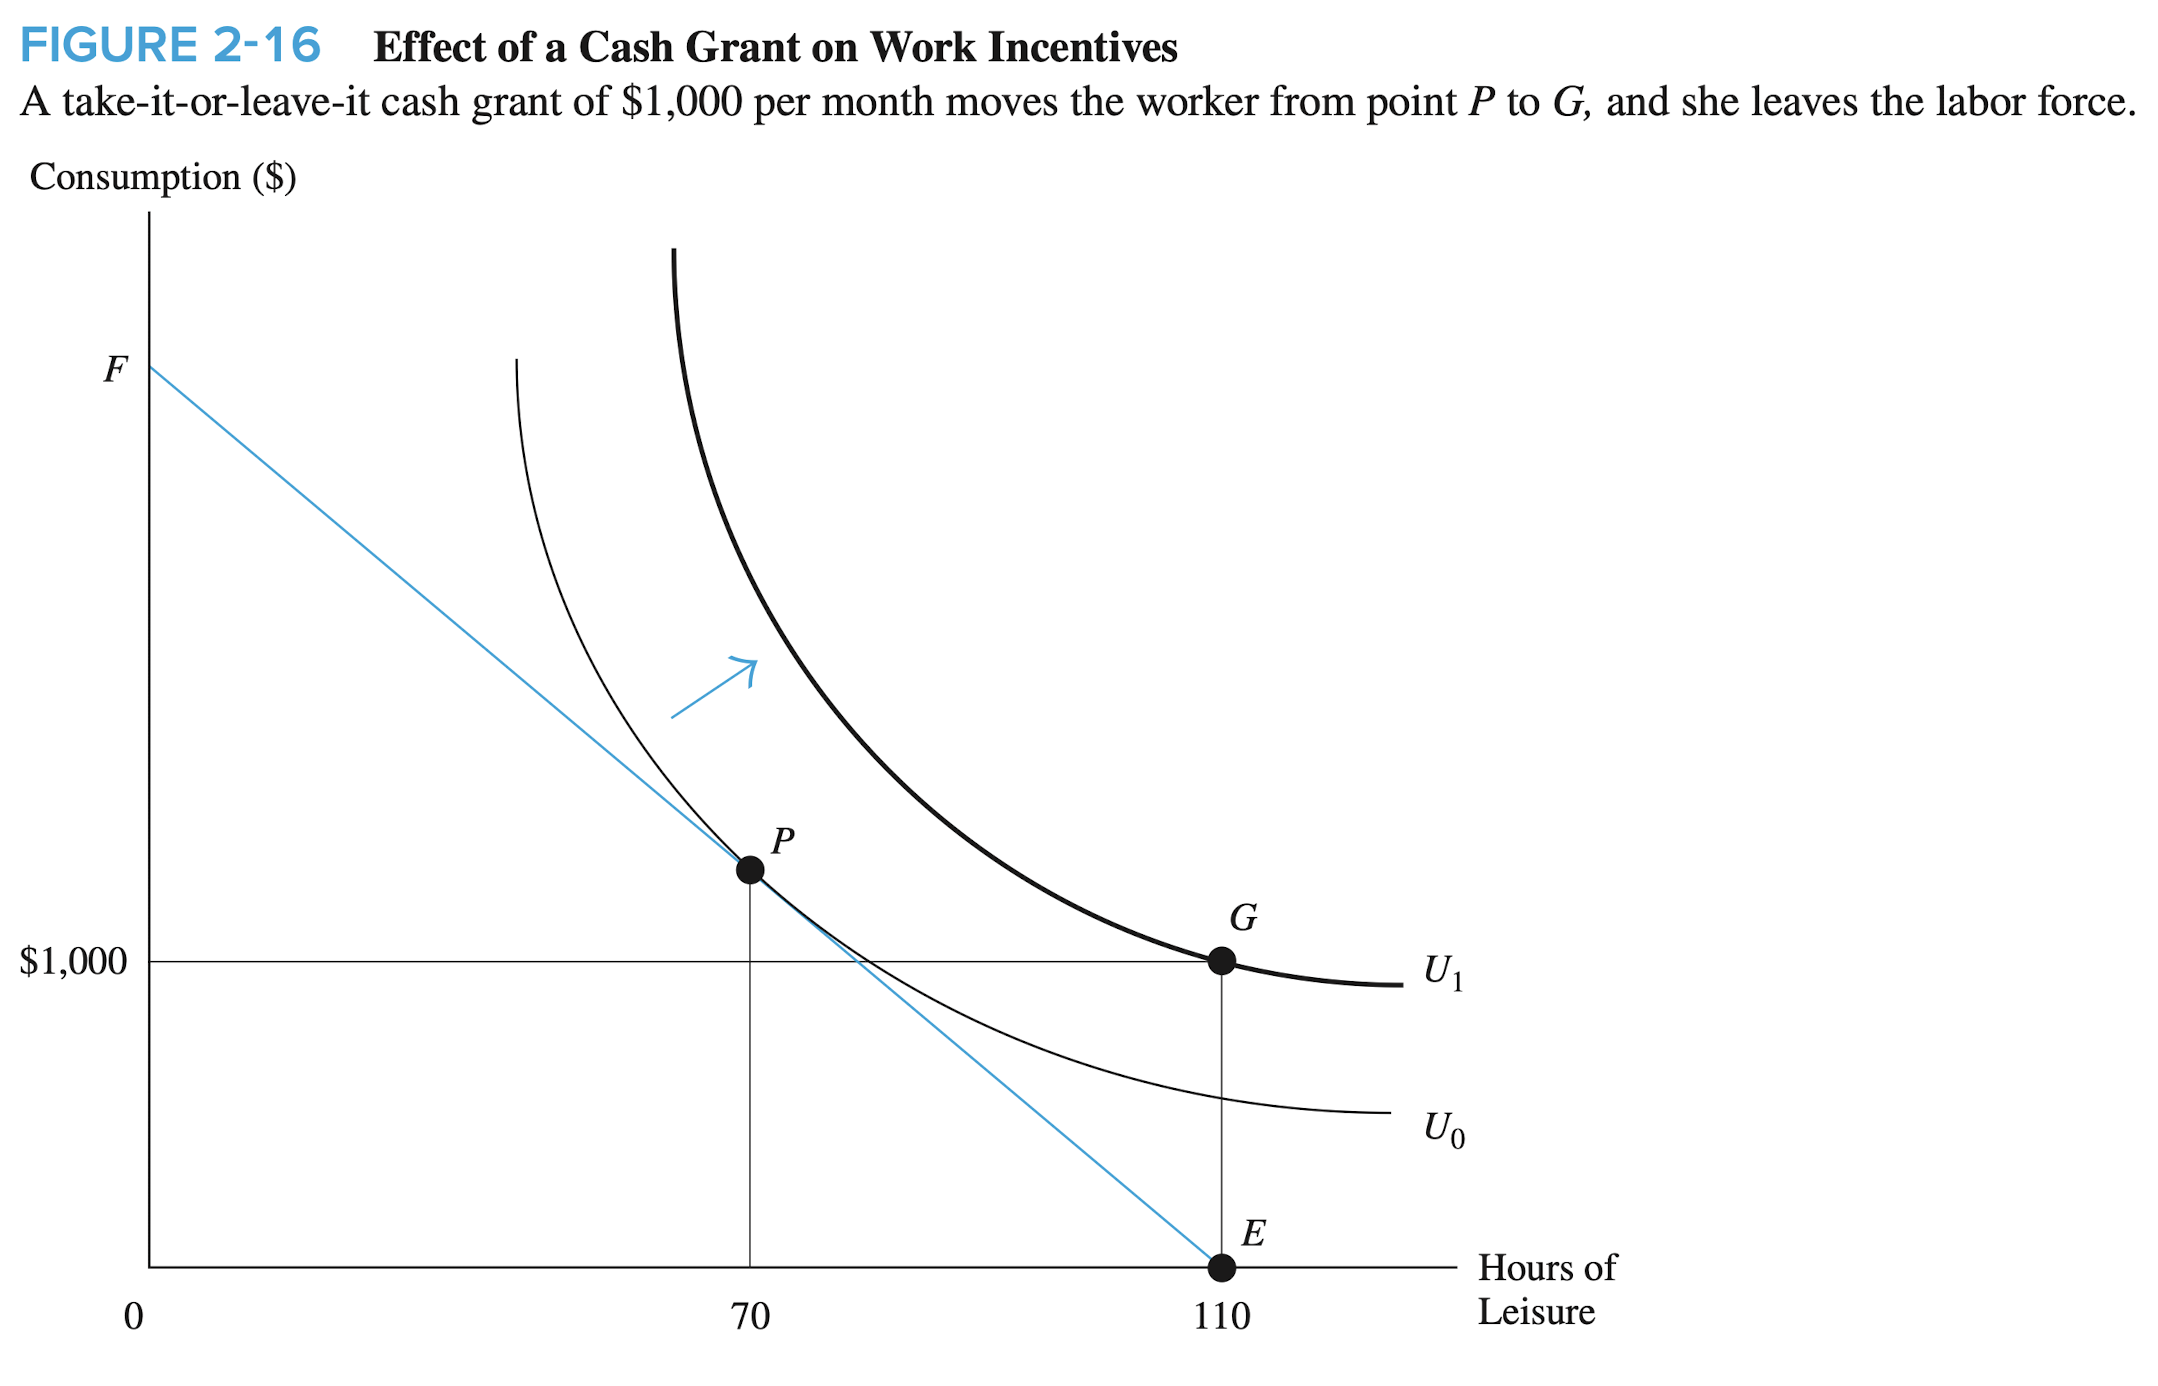
\includegraphics[width=0.9\textwidth]{../input/ch_2p11_cash_grant.png}
    \caption{The Effect of a Cash Grant on Labor Supply}
    \label{fig:ch2p11_cash_grant}
\end{figure}

\FloatBarrier

If we instead suppose that the worker receives 
a welfare benefit of \$$1,000$, which is then reduced 
by \$$0.50$ for every dollar earned in the market,
we can think of this as a 50\% tax on earnings for the first
\$$2,000$ of earnings.
An example of how this could play out for a worker 
is shown in \autoref{fig:ch2p11_welfare_hours_worked}.
As we can see, the policy shifts the opportunity set
from being characterized by $FE$ to $HG$, where 
$FE$ has a slope of $-1w$ and
$HG$ has a slope of $-0.5w$. The agent's choice is 
characterized by $P$ in the no-welfare scenario
and $R$ in the welfare scenario.
In this example, the income effect moves the worker
to $Q$, and the substitution effect then moves them to $R$.
In this example, the income and substitution effects work 
in the same direction, since the income effect makes the 
worker work less when labor is a normal good, and the 
substitution effect makes the worker work less, given that 
leisure is less expensive because of the effective tax on earnings.

\FloatBarrier

\begin{figure}[!htb]
    \centering
        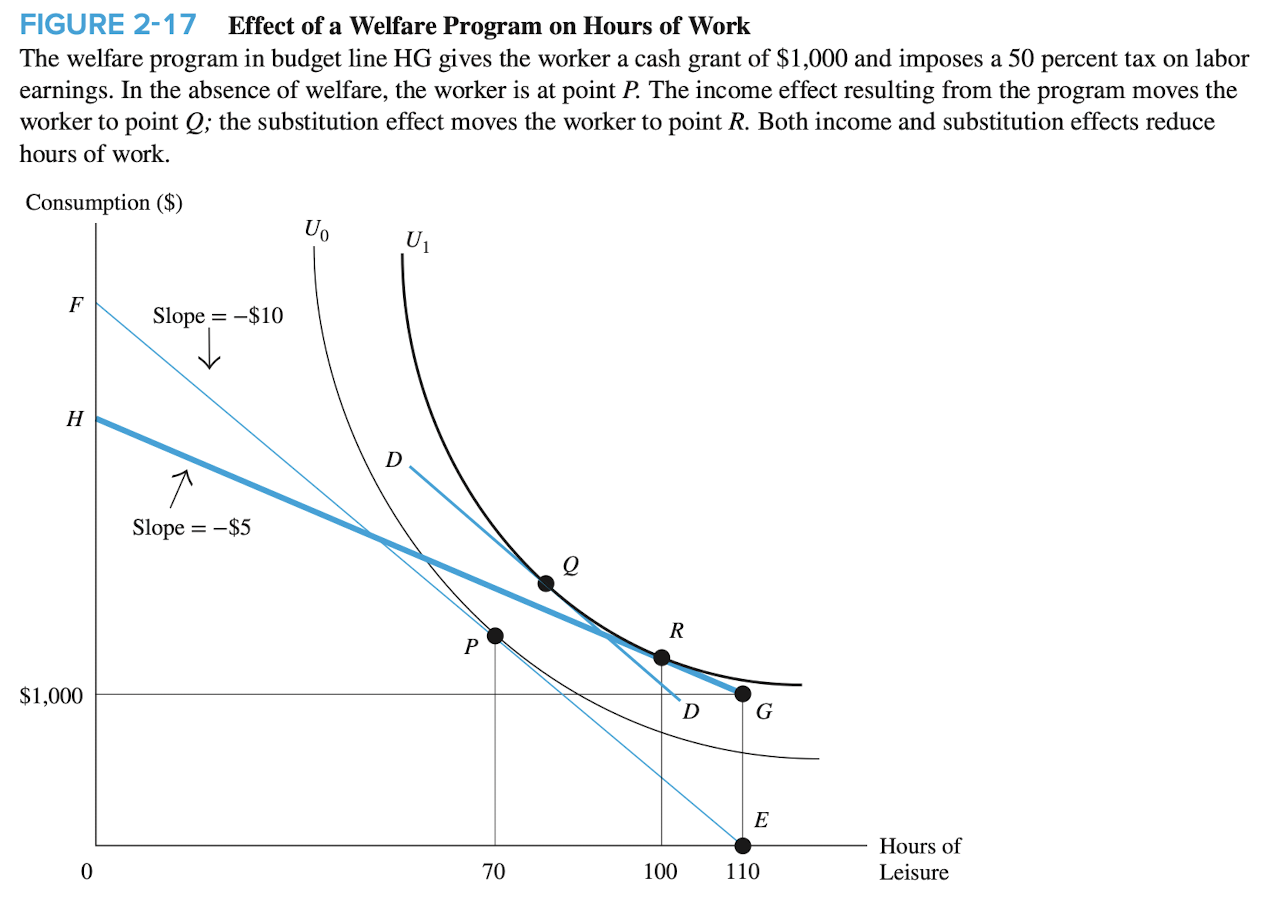
\includegraphics[width=0.9\textwidth]{../input/ch_2p11_welfare_hours_worked.png}
    \caption{The Effect of a Welfare Program on Labor Supply}
    \label{fig:ch2p11_welfare_hours_worked}
\end{figure}

\FloatBarrier

%%%%%%%%%%%%%%%%%%%%%%%%%%%%%%%%%%%%%%%%%%%%%%%%%%%%%%%%%%%%%%%%%%%%%%%%%%%%%%%%%%%%%%%
%%%%%%%%%%%%%%%%%%%%%%%%%%%%%%%%%%%%%%%%%%%%%%%%%%%%%%%%%%%%%%%%%%%%%%%%%%%%%%%%%%%%%%%
\subsection{Policy Application: The Earned Income Tax Credit}

The next example that we'll consider is the Earned Income Tax Credit (EITC).
The EITC is a subsidy for low-income working families.
The way that the EITC works is such that the workers earnings can be 
divided into four segments:
(1) on earnings up to $E_1$, 
a subsidy rate of $\tau$ applies, so that the 
worker earns $(1+\tau)w$ per hour worked;
(2) on earnings between $E_1$ and $E_2$,
the worker earns $w$ per hour worked;
(3) on earnings between $E_2$ and $E_3$,
the worker earns $(1-\rho)w$ per hour worked, where $\rho$ is
the phase-out rate; and
(4) on earnings above $E_3$, the worker earns $w$ per hour worked.
This is demonstrated graphically in \autoref{fig:ch2p12_eitc_structure}.

\FloatBarrier

\begin{figure}[!htb]
    \centering
        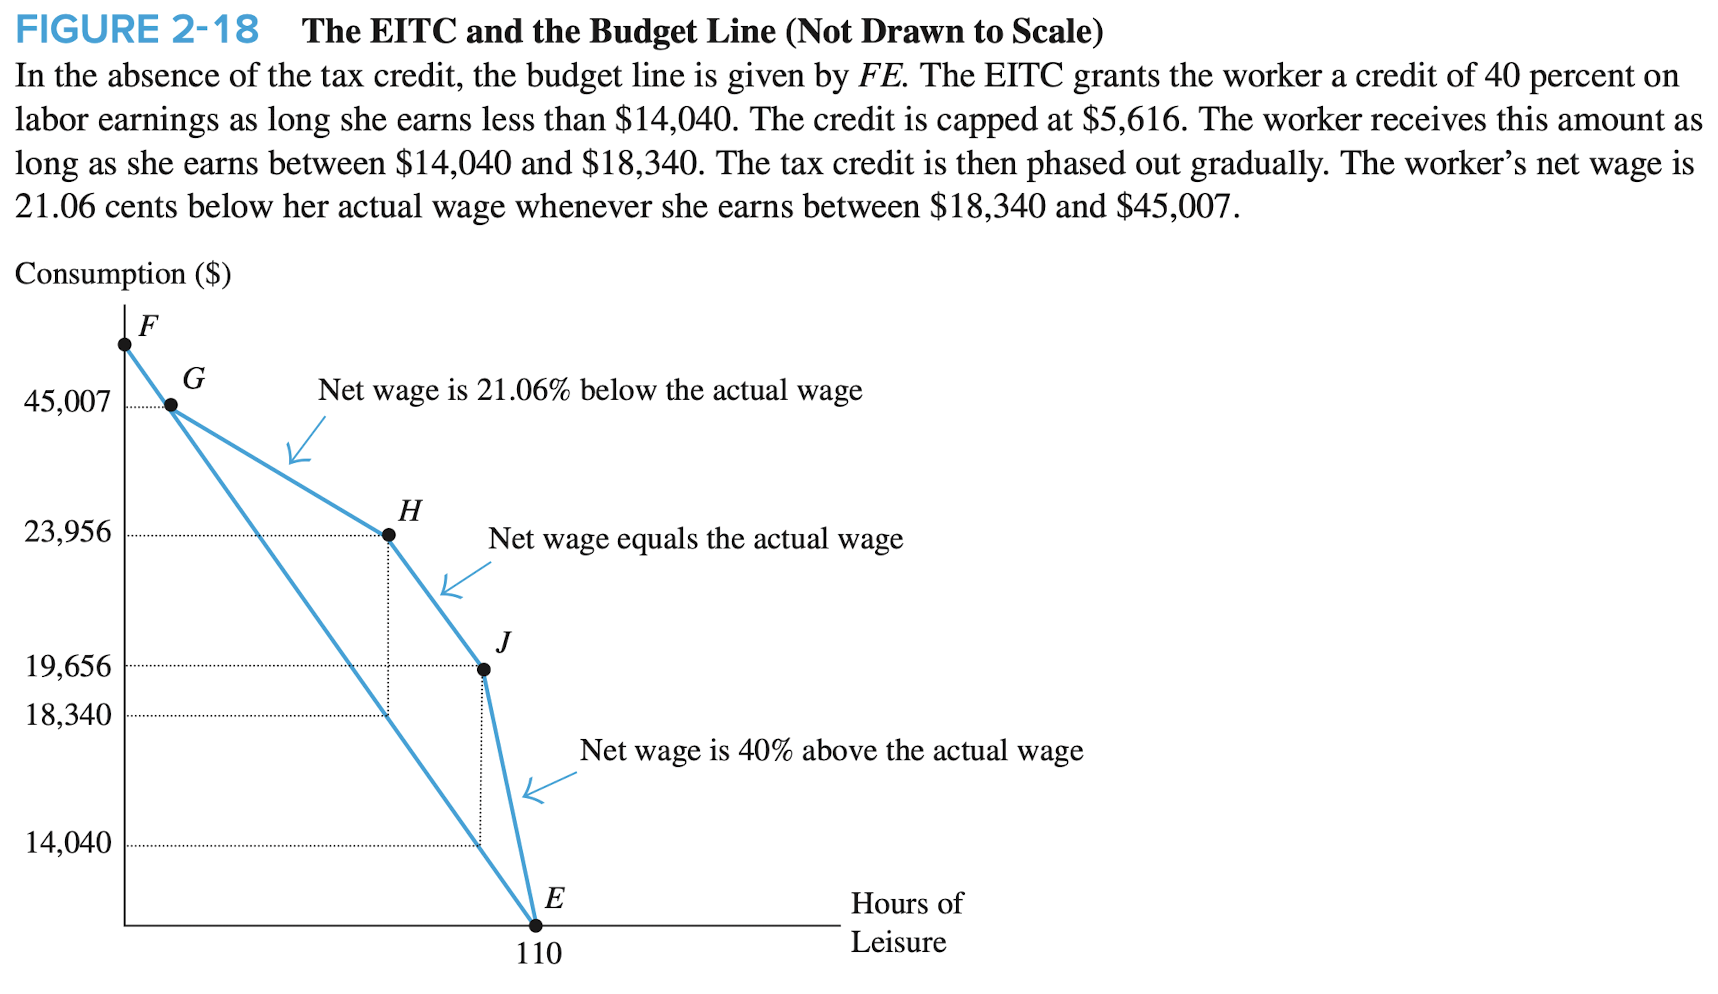
\includegraphics[width=0.9\textwidth]{../input/ch_2p12_eitc_structure.png}
    \caption{The Structure of the Earned Income Tax Credit}
    \label{fig:ch2p12_eitc_structure}
\end{figure}

\FloatBarrier

\autoref{fig:ch2p12_eitc_effects} demonstrates some possible 
effects of the EITC on a worker's labor supply. Panel (a)
demonstrates a worker who is brought into the labor force
by the EITC. Panel (b) demonstrates a worker who
reduces their hours worked due to the income effect of the EITC.
Panel (c) demonstrates a worker who decreases their hours worked 
due to the income and substitution effects of the EITC.


\FloatBarrier

\begin{figure}[!htb]
    \centering
        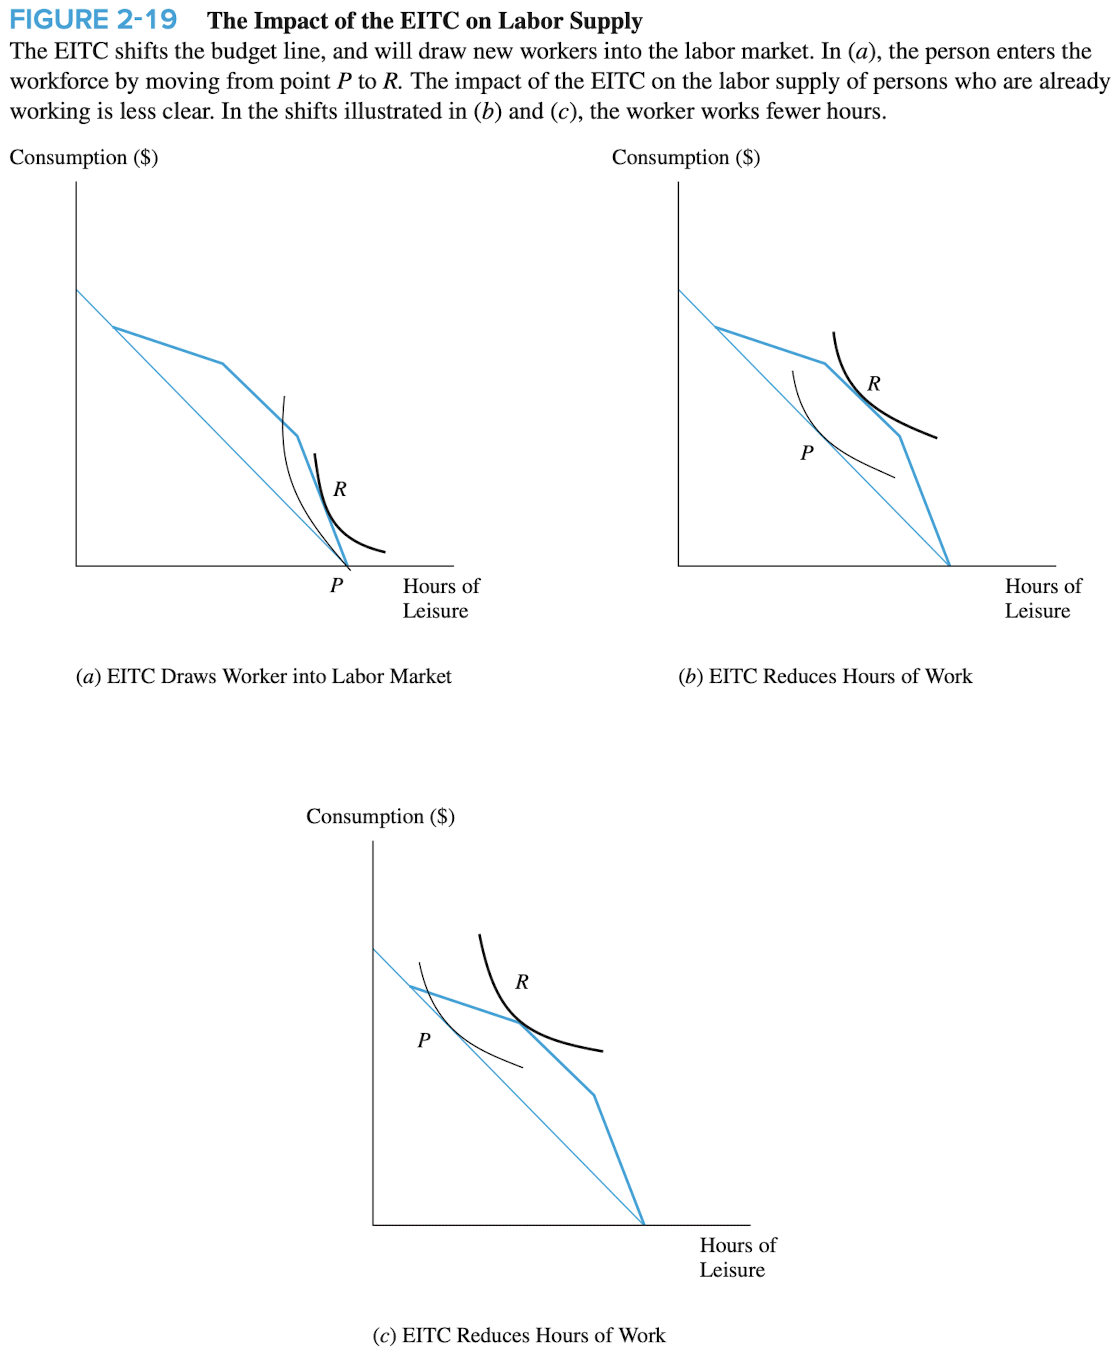
\includegraphics[width=0.9\textwidth]{../input/ch_2p12_eitc_effects.png}
    \caption{The Effects of the Earned Income Tax Credit}
    \label{fig:ch2p12_eitc_effects}
\end{figure}

\FloatBarrier

%%%%%%%%%%%%%%%%%%%%%%%%%%%%%%%%%%%%%%%%%%%%%%%%%%%%%%%%%%%%%%%%%%%%%%%%%%%%%%%%%%%%%%%
%%%%%%%%%%%%%%%%%%%%%%%%%%%%%%%%%%%%%%%%%%%%%%%%%%%%%%%%%%%%%%%%%%%%%%%%%%%%%%%%%%%%%%%
\subsection{Labor Supply Over the Life Cycle}

Consumption and leisure decisions are made over the course of the life cycle. 
Thus, workers can shift their labor to periods of relative higher productivity.
This hypothesis is known as the ``intertemporal substitution hypothesis.''
\autoref{fig:ch2p13_life_cycle} illustrates the typical earnings and hours worked
patterns over the life cycle. Models of life cycle labor supply
crucially depend on estimating the intertemporal 
labor supply elasticity. I won't include so much more discussion of this 
right now.

\FloatBarrier

\begin{figure}[!htb]
    \centering
        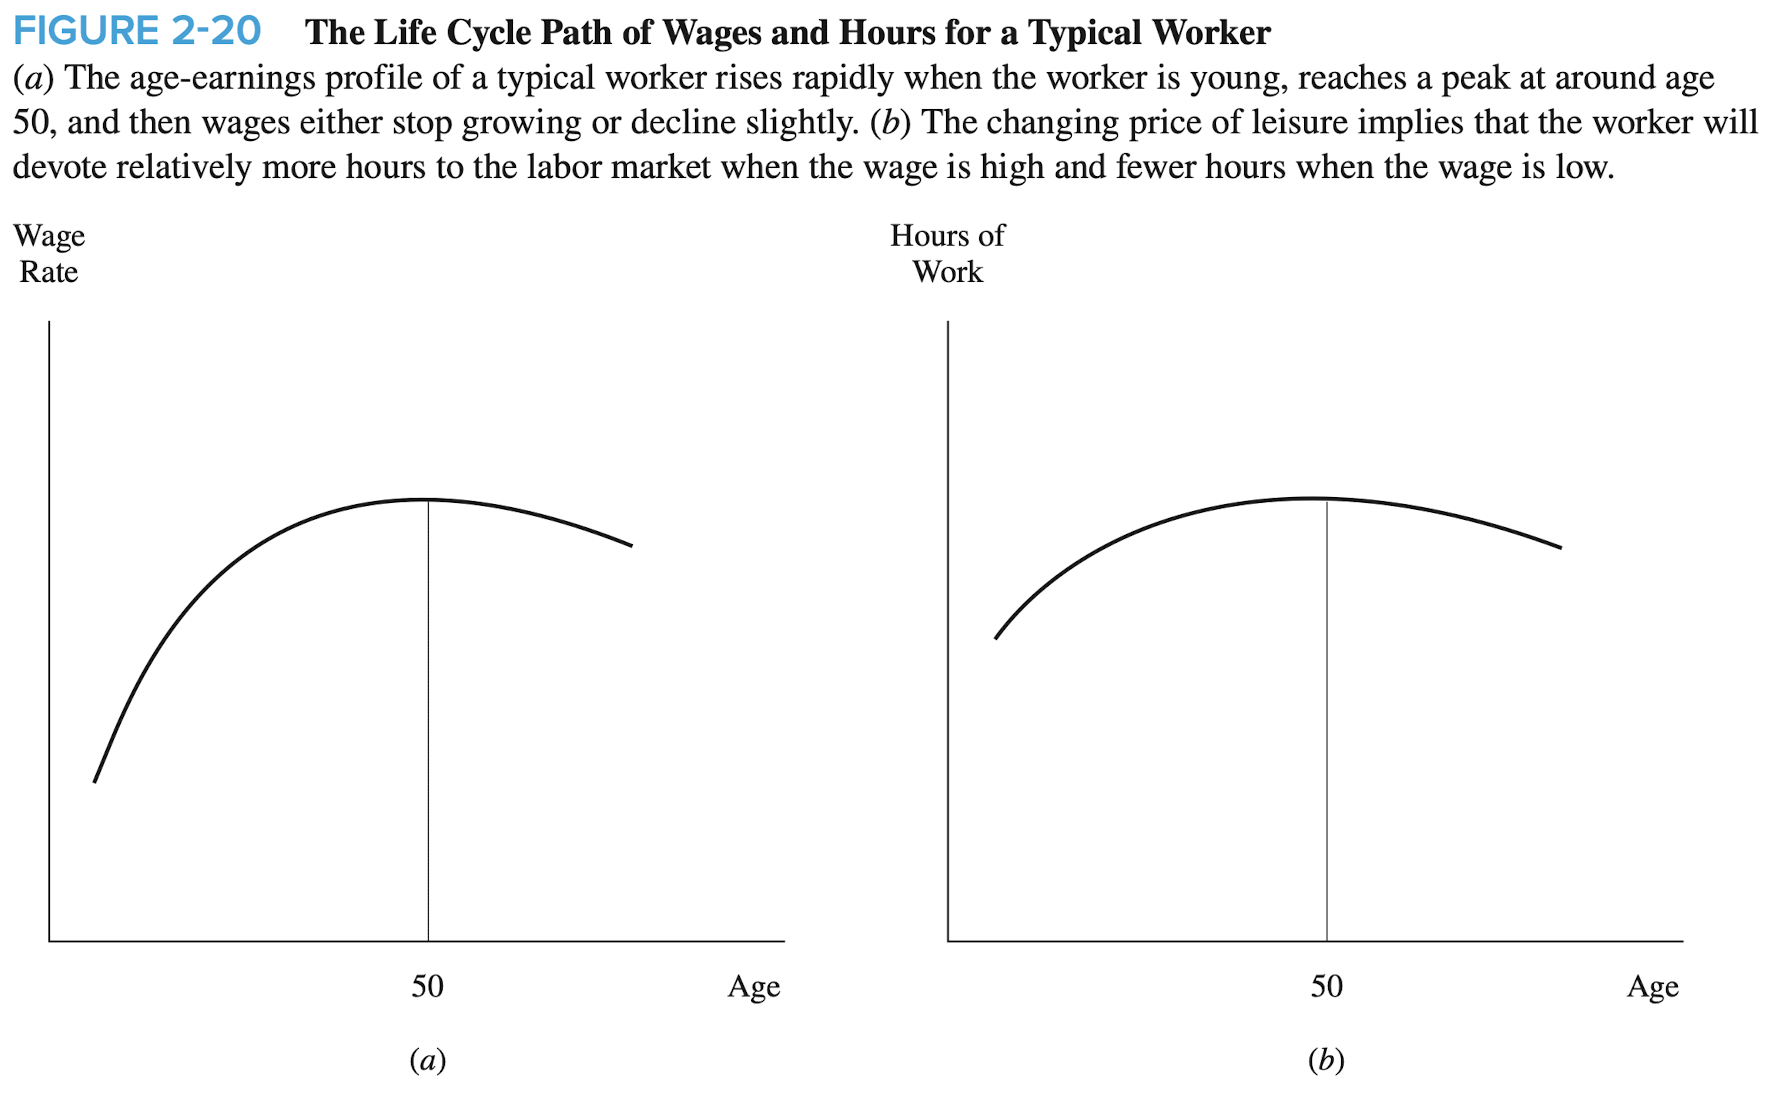
\includegraphics[width=0.9\textwidth]{../input/ch_2p13_life_cycle.png}
    \caption{Wages and Hours Worked Over the Life Cycle}
    \label{fig:ch2p13_life_cycle}
\end{figure}

\FloatBarrier

%%%%%%%%%%%%%%%%%%%%%%%%%%%%%%%%%%%%%%%%%%%%%%%%%%%%%%%%%%%%%%%%%%%%%%%%%%%%%%%%%%%%%%%
%%%%%%%%%%%%%%%%%%%%%%%%%%%%%%%%%%%%%%%%%%%%%%%%%%%%%%%%%%%%%%%%%%%%%%%%%%%%%%%%%%%%%%%
\subsection{Policy Application: Disability Benefits and Labor Force Participation}

The textbook then discusses some evidence that 
disability benefits reduce labor force participation.
In particular, the author discusses some research suggesting that people 
who get denied disability benefits are more likely to work
afterwards than people who are approved, even 
after attempting to sort through the endogeneity 
issues (e.g., by using an instrumental variable approach).
I don't doubt that these results are true, but I'm not really sure 
what I'm meant to take away from it in a normative sense. Perhaps nothing.